\documentclass[spanish,a4paper,12pt,oneside,notitlepage]{extreport}

%%%%%%%%%%%%%%%%%%%%%%%%%%%%%%%%%%%%%%%%%%%%%%%%%%%%%%%%%%%%%%%%%%%%%%%%%%%%%%%
\usepackage{graphicx}
\usepackage{epsfig}
\usepackage[utf8]{inputenc}
\usepackage[spanish]{babel}
\usepackage{alltt}
\usepackage{algorithm}
\usepackage{algorithmic}
\usepackage{multirow}
\usepackage[top=3cm, bottom=3cm, left=3cm, right=3cm]{geometry}
\usepackage{libertinus}
\usepackage[T1]{fontenc}
\usepackage{titlesec}
\usepackage{csquotes}
% \usepackage[ttdefault=true]{AnonymousPro}
\usepackage[font=small,labelfont=bf]{caption}
\usepackage{setspace}
\usepackage[labelfont=bf]{subcaption}
\usepackage[dvipsnames]{xcolor}
\usepackage{url}
\usepackage{listings}
\usepackage{hyperref}
\usepackage{wrapfig}
\usepackage{lipsum}

\usepackage{courier}
\lstset{basicstyle=\footnotesize\ttfamily,breaklines=true}

\usepackage[style=numeric,sorting=none]{biblatex}
\addbibresource{report.bib}
 
\setcounter{secnumdepth}{3}
\setcounter{tocdepth}{3}
 
\captionsetup{font={small,stretch=0.95}}
 
\newcommand{\SONY}{{\sc Sony}}
\newcommand{\MICROSOFT}{{\sc Microsoft}}
\newcommand{\GCC}{\textsf{\textsc{G}CC}}
\newcommand{\INTEL}{\textsf{\textsc{I}ntel}}

%%% Traducimos el pseudocodigo
\renewcommand{\algorithmicwhile}{\textbf{mientras}}
\renewcommand{\algorithmicend}{\textbf{fin}}
\renewcommand{\algorithmicdo}{\textbf{hacer}}
\renewcommand{\algorithmicif}{\textbf{si}}
\renewcommand{\algorithmicthen}{\textbf{entonces}}
\renewcommand{\algorithmicrepeat}{\textbf{repetir}}
\renewcommand{\algorithmicuntil}{\textbf{hasta que}}
\renewcommand{\algorithmicelse}{\textbf{en otro caso}}
\renewcommand{\algorithmicfor}{\textbf{para}}

%\newcommand{\RETURN}{\textbf{retornar} }
\newcommand{\RET}{\STATE \textbf{retornar} }
\newcommand{\TO}{\textbf{hasta} }
\newcommand{\AND}{\textbf{y} }
\newcommand{\OR}{\textbf{o} }

\renewcommand{\baselinestretch}{1.1} 


%%%%%%%%%%%%%%%%% Creamos un entorno para listar código fuente %%%%%%%%%%%%%%%
\newenvironment{sourcecode}
{\begin{list}{}{\setlength{\leftmargin}{1em}}\item\scriptsize\bfseries}
{\end{list}}

\newenvironment{littlesourcecode}
{\begin{list}{}{\setlength{\leftmargin}{1em}}\item\tiny\bfseries}
{\end{list}}

\newenvironment{summary}
{\par\noindent\begin{center}\textbf{Abstract}\end{center}\begin{itshape}\par\noindent}
{\end{itshape}}

\newenvironment{keywords}
{\begin{list}{}{\setlength{\leftmargin}{1em}}\item[\hskip\labelsep \bfseries Keywords:]}
{\end{list}}

\newenvironment{palabrasClave}
{\begin{list}{}{\setlength{\leftmargin}{1em}}\item[\hskip\labelsep \bfseries Palabras clave:]}
{\end{list}}


%%%%%%%%%%%%%%%%%%%%%%%%%%%%%%%%%%%%%%%%%%%%%%%%%%%%%%%%%%%%%%%%%%%%%%%%%%%%%%%
% Format
%%%%%%%%%%%%%%%%%%%%%%%%%%%%%%%%%%%%%%%%%%%%%%%%%%%%%%%%%%%%%%%%%%%%%%%%%%%%%%%
%\usepackage{showframe}
%\marginparwidth 0mm
%%\topmargin -4 mm
%\topmargin -21 mm
%\headheight 10 mm
%\headsep 10 mm

%\textheight 229 mm
%\textheight 246 mm

%\oddsidemargin -5.4 mm
%\evensidemargin -5.4 mm
%\oddsidemargin 5 mm
%\evensidemargin 5 mm

%\oddsidemargin -3 mm
%\evensidemargin -3 mm

%\textwidth 17 cm
%\textwidth 15 cm
%\columnsep 10 mm

\input{amssym.def}

%%%%%%%%%%%%%%%%%%%%%%%%%%%%%%%%%%%%%%%%%%%%%%%%%%%%%%%%%%%%%%%%%%%%%%%%%%%%%%%

\begin{document}

%%%%%%%%%%%%%%%%%%%%%%%%%%%%%%%%%%%%%%%%%%%%%%%%%%%%%%%%%%%%%%%%%%%%%%%%%%%%%%%
% First Page
%%%%%%%%%%%%%%%%%%%%%%%%%%%%%%%%%%%%%%%%%%%%%%%%%%%%%%%%%%%%%%%%%%%%%%%%%%%%%%%

\pagestyle{empty}
\thispagestyle{empty}

\newcommand{\HRule}{\rule{\linewidth}{1mm}}
\setlength{\parindent}{0mm}
\setlength{\parskip}{0mm}


\vspace*{\stretch{0.3}}
\begin{center}
  % \includegraphics[scale=0.8]{images/logo_vertical}\\[10mm]
  
\includegraphics[scale=1]{images/logo-esit}\\[10mm]
  \vspace*{\stretch{0.5}}
  {\huge \scshape Trabajo de Fin de Grado}
\end{center}

\HRule
\begin{center}
  \vspace{1em}
  {\Huge Planificación optimizada de un sistema de semáforos mediante algoritmos evolutivos: una aplicación a la rotonda del Padre Anchieta, en Santa Cruz de Tenerife} \\[3mm]
  \rule{5cm}{0.6pt}\\[5mm]
  {\Large \textit{Optimized planning of a traffic light system using evolutionary algorithms: an application to the Padre Anchieta roundabout, in Santa Cruz de Tenerife}} \\[3mm]
  \rule{5cm}{0.6pt}\\[5mm]
  {\Large Francisco Arturo Cruz Zelante}
\end{center}
\HRule

\vspace*{\stretch{2}}

\begin{center}
  \Large San Cristóbal de La Laguna, \today
\end{center}

\titleformat{\chapter}[display]
{\normalfont%
    \LARGE% %change this size to your needs for the first line
    \itshape}{\chaptertitlename\ \thechapter}{20pt}{%
    \normalfont \bfseries \Huge %change this size to your needs for the second line
}


%%%%%%%%%%%%%%%%%%%%%%%%%%%%%%%%%%%%%%%%%%%%%%%%%%%%%%%%%%%%%%%%%%%%%%%%%%%%%%%
\newpage{\pagestyle{empty}}
\thispagestyle{empty}
%%%%%%%%%%%%%%%%%%%%%%%%%%%%%%%%%%%%%%%%%%%%%%%%%%%%%%%%%%%%%%%%%%%%%%%%%%%%%%%

% \pagestyle{myheadings} %my head defined by markboth or markright
% % No funciona bien \markboth sin "twoside" en \documentclass, pero al
% % ponerlo se dan un montón de errores de underfull \vbox, con lo que no se
% % ha puesto.
% \markboth{Francisco Arturo Cruz Zelante}{Planificación optimizada de un sistema de semáforos mediante algoritmos evolutivos: una aplicación a la rotonda del Padre Anchieta, en Santa Cruz de Tenerife}

%Numeracion en romanos
\renewcommand{\thepage}{\roman{page}}
\setcounter{page}{1}

\newpage{\pagestyle{empty}}
\thispagestyle{empty}

\chapter*{}
\begin{flushright}
    {\Huge\textbf{Agradecimientos}}
    \bigskip
    \bigskip

    {\itshape
        Aquí van los agradecimientos
    }
\end{flushright}


\newpage{\pagestyle{empty}}
\thispagestyle{empty}
\pagestyle{empty}

\begin{center}
    \textbf{Resumen}
\end{center}

El resumen es una síntesis del contenido esencial del TFG/TFM, una representación abreviada y precisa del contenido del documento, sin interpretación ni crítica, que ayuda al lector a decidir la lectura o no del texto completo. El resumen debe reflejar los objetivos, la metodología, los resultados y las conclusiones más importantes del TFG/TFM, empleando una terminología normalizada de la materia. Características del resumen: Brevedad. La extensión debe estar entre las 150-200 palabras. Autonomía. El resumen tiene que ser un texto coherente y se tiene que entender por sí solo, de forma independiente del texto base. Precisión. Debe recoger los conceptos más importantes del documento. Claridad. El resumen debe ser comprensible, sencillo e informativo. Fidelidad al TFG/TFM original. El resumen ha de reflejar el contenido del original, sin introducir variaciones, ni interpretaciones.


\medskip

\noindent \textbf{Palabras clave:} SUMO, simulación, tráfico, algoritmos evolutivos, TypeScript, semáforos, planificación, optimización

\bigskip
\bigskip

\begin{center}
    \textbf{Abstract}
\end{center}

The summary is a synthesis of the essential content of the TFG/TFM, an abbreviated and precise representation of the document's content, without interpretation or criticism, which helps the reader to decide whether or not to read the full text. The summary should reflect the objectives, methodology, results and main conclusions of the TFG/TFM, using standardized subject matter terminology. Characteristics of the summary: Brevity. The length should be between 150-200 words. Autonomy. The abstract must be a coherent text and must be understood on its own, independently of the base text. Accuracy. It must include the most important concepts of the document. Clarity. The summary must be understandable, simple and informative. Fidelity to the original TFG/TFM. The summary must reflect the content of the original, without introducing variations or interpretations.

\medskip

\noindent \textbf{Keywords:} SUMO, traffic, simulation, evolutionary algorithms, TypeScript, traffic lights, scheduling, optimization



\tableofcontents

\newpage{\pagestyle{empty}}
\listoffigures

\newpage{\pagestyle{empty}}
\listoftables

\newpage{\pagestyle{empty}}

% \setlength{\parindent}{6mm}
\setlength{\parskip}{4mm}

%Numeracion a partir del capitulo I
\renewcommand{\thepage}{\arabic{page}}
\setcounter{page}{1}
\pagestyle{plain}

\chapter{Introducción}
\label{cap:1-intro}

La rotonda de Padre Anchieta (cuyo nombre real es «glorieta del Brasil») toma su nombre por la escultura, regalada por el pueblo brasileño, colocada en el centro de la rotonda en representación del beato José de Anchieta~\cite{gallo_glorieta_2013}.

% Gara: Aquí vendría bien una imagen del Padre Anchieta
\begin{figure}[H]
    \centering
    \includegraphics[width=\textwidth]{report/images/padre-anchieta.png}
    \caption[Mapeado en 3D de la Rotonda del Padre Anchieta.]{Mapeado en 3D de la Rotonda del Padre Anchieta. Cortesía de Google Earth\protect\footnotemark}
    \label{fig:padre_anchieta_3d}
\end{figure}

\footnotetext{Véase \url{https://earth.google.com/web/@28.48023943,-16.31770104,534.93762391a,251.9187181d,35y,-46.25428648h,74.81244137t,0r}}

La popularidad de la rotonda se explica por su posición estratégica, rodeada de viviendas, comercios, dos campus universitarios de la Universidad de La Laguna (Central y Anchieta), y por la cual pasa una de las principales autopistas de la isla, la TF-5; además de conectar otras cuatro vías: la Carretera de la Esperanza (TF-24), la Carretera de Geneto (TF-263), la Avenida de la Trinidad y la Avenida Astrofísico Francisco Sánchez. Sin embargo, los orígenes de la rotonda son considerablemente más humildes (véase la Figura~\ref{fig:anchieta_ev}).

El tráfico que asume la rotonda es muy considerable, especialmente en horas punta, hasta tal punto en que se producen retenciones muy importantes y, en determinadas situaciones, un bloqueo total del tráfico, a veces durante horas (véase~\cite{gulesserian_vuelven_2018}, a modo de ejemplo). Las grandes cantidades de tráfico que absorbe la rotonda, y los bloqueos y ralentizaciones que se producen como consecuencia, tienden a afectar al tráfico de la TF-5, causando retenciones a la altura de la rotonda.

La optimización del tráfico en la rotonda se convierte, por tanto, en un asunto de primer orden respecto de la movilidad en la isla. La rotonda da una vía a los estudiantes tanto del norte como del sur que van a clase, a los trabajadores que se dirigen hacia La Laguna y hacia Santa Cruz; y en general a una gran cantidad de trayectos entre ambas ciudades y el norte de la isla que no puede dejarse desatendida.

\begin{figure}[h]
    \centering
    \begin{subfigure}[t]{.49\textwidth}
      \centering
      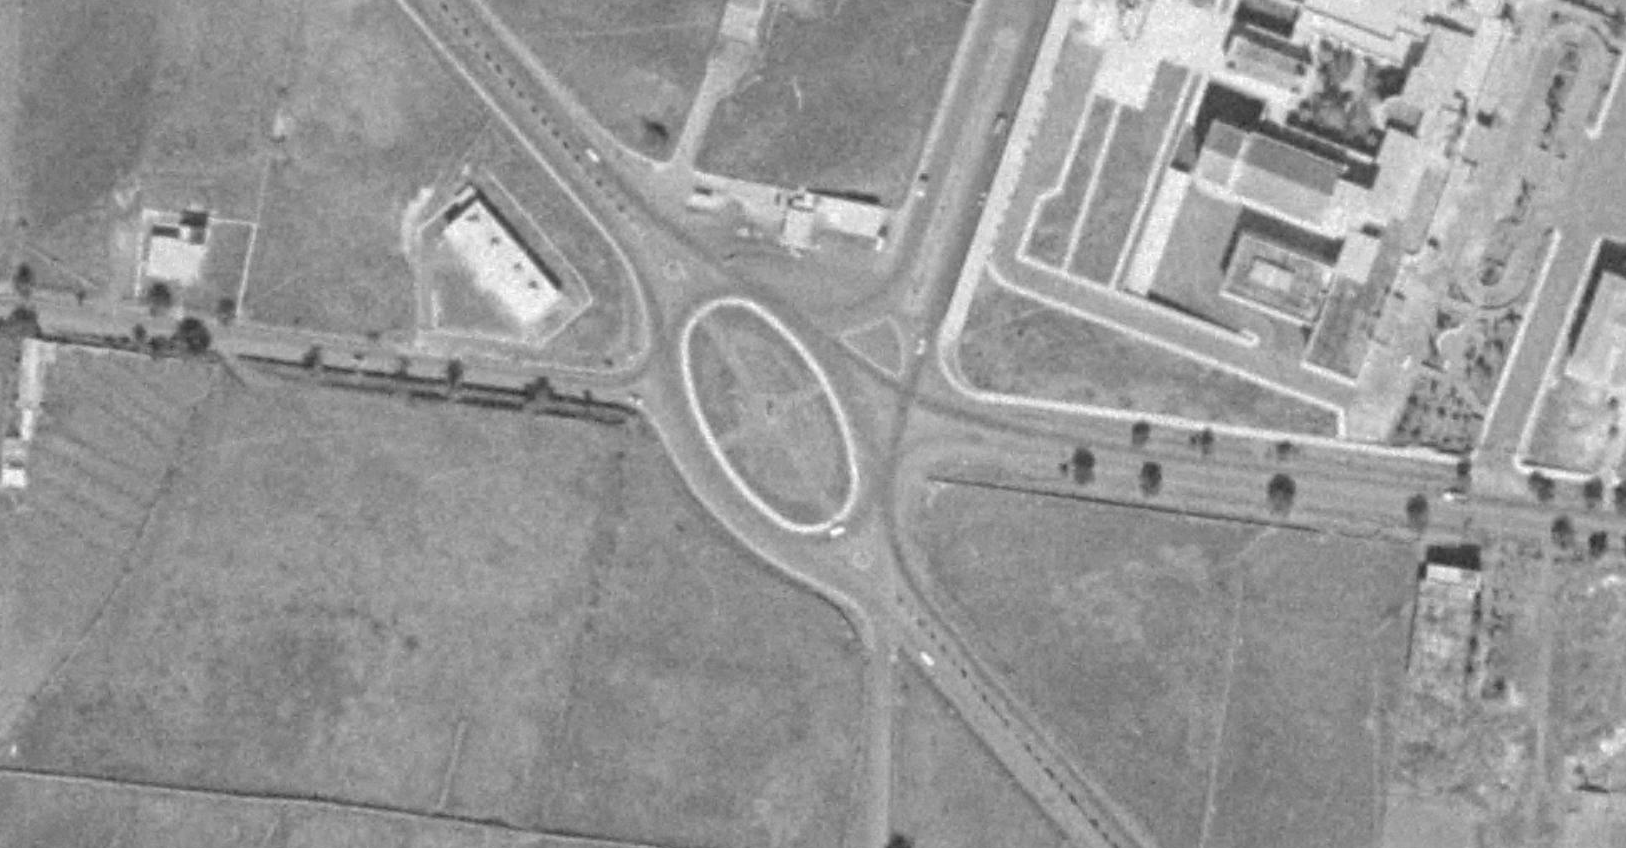
\includegraphics[width=\textwidth]{report/images/amp-anchieta-1964.png}
      \caption{1964}
      \label{fig:anchieta1964}
    \end{subfigure}
    \hfill
    \begin{subfigure}[t]{.49\textwidth}
      \centering
      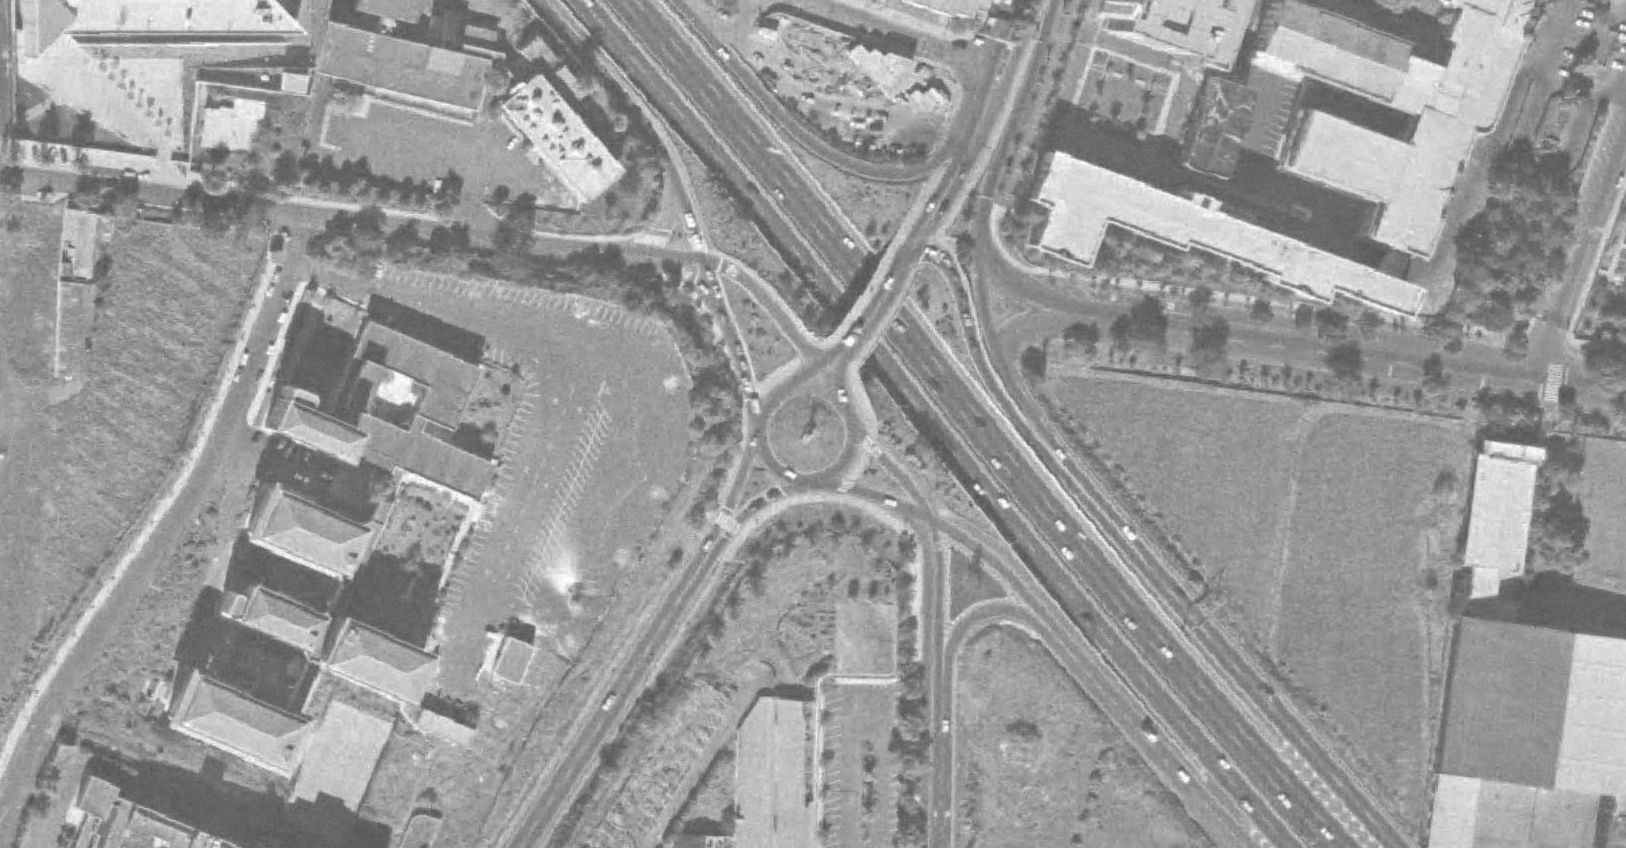
\includegraphics[width=\textwidth]{report/images/amp-anchieta-1994.png}
      \caption{1994}
      \label{fig:anchieta1994}
    \end{subfigure}
    \vspace{0.7cm}
    \begin{subfigure}[t]{.49\textwidth}
      \centering
      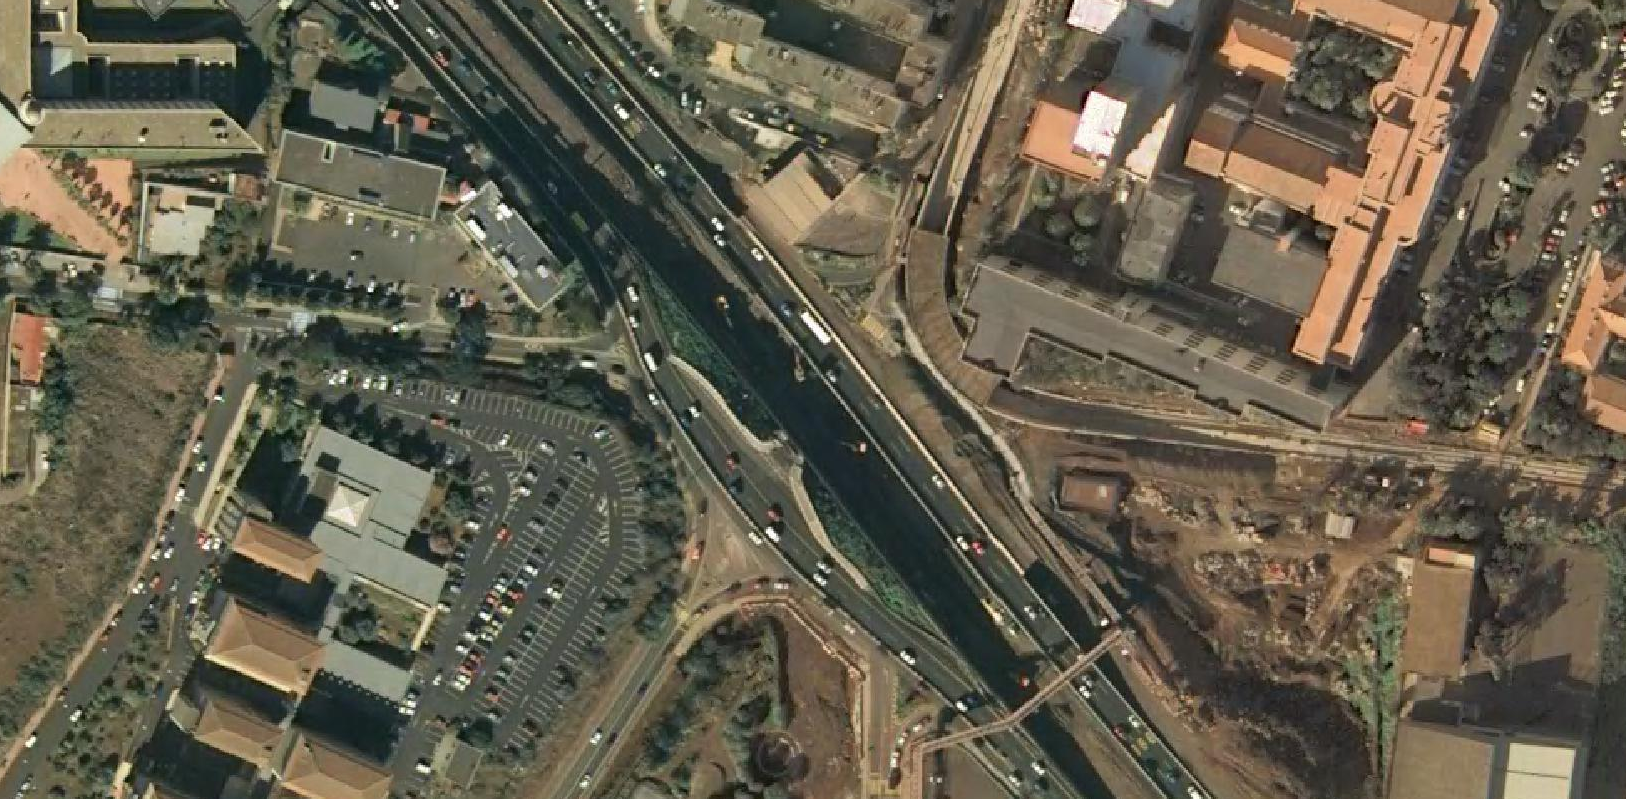
\includegraphics[width=\textwidth]{report/images/amp-anchieta-2006.png}
      \caption{2006 (en obras)}
      \label{fig:anchieta2006}
    \end{subfigure}
    \hfill
    \begin{subfigure}[t]{.49\textwidth}
      \centering
      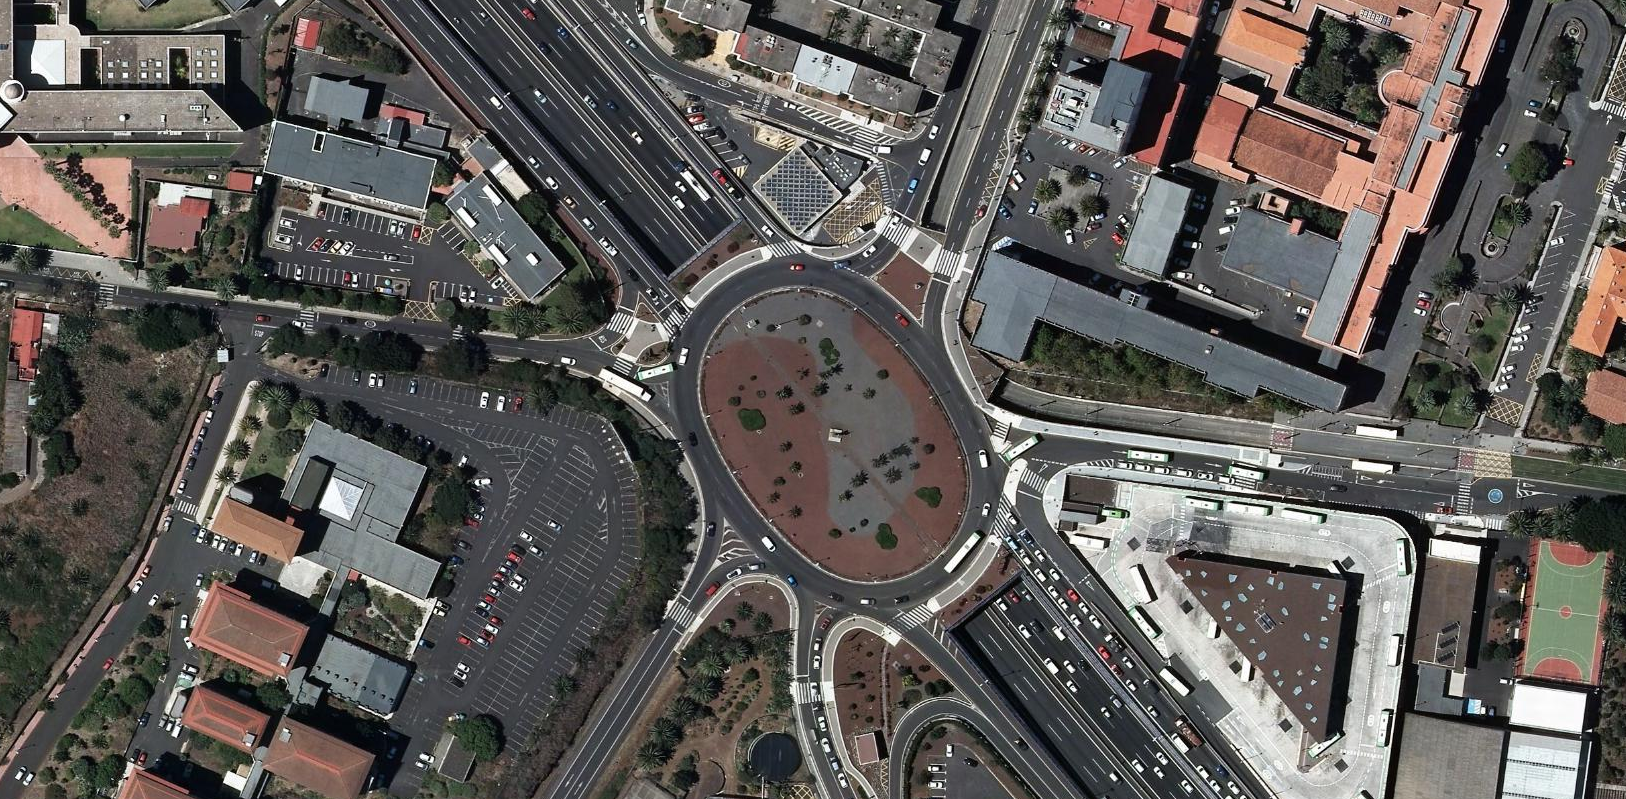
\includegraphics[width=\textwidth]{report/images/amp-anchieta-2019.png}
      \caption{2019}
      \label{fig:anchieta2019}
    \end{subfigure}
    \caption[Evolución de la rotonda de Padre Anchieta a lo largo de los años.]{Evolución de la rotonda de Padre Anchieta a lo largo de los años. Fotografías cortesía de GRAFCAN\protect\footnotemark}
    \label{fig:anchieta_ev}
\end{figure}

\footnotetext{Véase \url{https://visor.grafcan.es/visorweb/}}

Las autoridades de la isla no son ajenas al problema de tráfico que plantea de la rotonda. El Cabildo de Tenerife, organismo de cuya competencia depende la rotonda, y el Gobierno de Canarias, de cuya competencia depende la TF-5, han planteado varias medidas, de entre las cuales cabe mencionar:

\begin{itemize}
    \item El soterramiento de la TF-24 en dirección hacia Santa Cruz (a la espera de ejecutar el proyecto)~\cite{dia_cabildo_2019}.
    \item La construcción de una pasarela de peatones sobre la rotonda~\cite{rozas_pasarela_2019}.
    \item La potenciación del vehículo compartido y el transporte público: creación de carriles BUS-VAO en la TF-5~\cite{20minutos_gobierno_2019}.
    \item Las propuestas para la construcción de nuevas líneas de tranvía~\cite{redaccion_de_eldiarioes_cabildo_2020}.
\end{itemize}

Sin embargo, todas las medidas mencionadas suponen un cargo importante al erario público, suponen una carga administrativa importante (por todos los procesos de licitación y control que han de realizarse), llevan mucho tiempo construirlas y mientras dure el proceso resultarán un incordio para los conductores y usuarios de la vía.


\section{Objetivos}

Con la elaboración de este proyecto lo que se propone es la instalación de semáforos en la rotonda, cuyas duraciones de fase se optimicen mediante un algoritmo evolutivo. De esta forma, se podrá comprobar si con la instalación de estos semáforos es posible mejorar la circulación del tráfico en función de determinados parámetros como: la duración media de los trayectos de los vehículos, la velocidad media de los vehículos, la cantidad de vehículos que han logrado completar su trayecto en una hora, etc.

El problema que se pretende abordar no es otro que el de la planificación de la duración de las fases de los semáforos, más conocido como el \textit{Traffic Light Scheduling Problem} (TLSP). Este problema de optimización plantea cuánto deberían durar las fases de los semáforos de uno o varios cruces para mejorar la circulación con respecto a varios parámetros; el más habitual de ellos siendo el tiempo medio de viaje de un grupo de vehículos desde un origen hasta el destino. Otros parámetros, como la distancia media o la contaminación de los vehículos también pueden ser tenidos en cuenta a la hora de evaluar el comportamiento de las distintas configuraciones semafóricas.

\begin{figure}[!t]
    \centering
    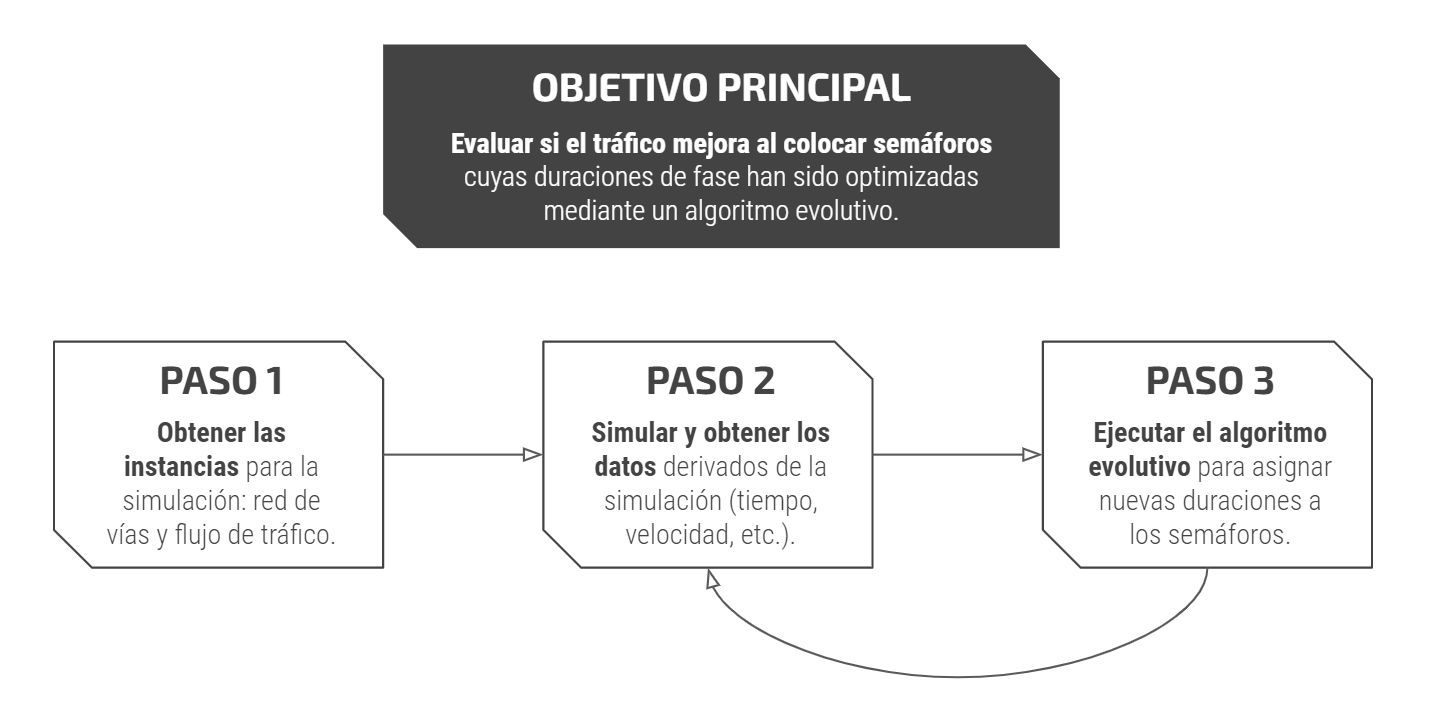
\includegraphics[width=\textwidth]{report/images/evolutionary_alg_graph.png}
    \caption{Gráfica del proceso general del trabajo.}
    \label{fig:evolutionary_alg_graph}
\end{figure}

En comparación con las medidas antes mencionadas, la que se propone en este trabajo supone un coste considerablemente más bajo, no molestaría tanto a los conductores durante la instalación (la cual sería también mucho más corta y sencilla) y plantea una solución muy interesante que podría ser reaprovechado para otras vías sin coste alguno (si ya tuvieran semáforos instalados).

Para llevar a cabo el proyecto, se han empleado principalmente las dos herramientas siguientes:

\begin{itemize}
    \item La primera de ellas es \textit{SUMO}~\cite{lopez_microscopic_2018}, un simulador de tráfico microscópico que nos permitirá evaluar cómo se comporta el tráfico en la rotonda de Padre Anchieta, con datos de tráfico provistos por el Cabildo de Tenerife.
    \item La segunda es \textit{Genetics.js}~\cite{abrante_dorta_framework_2019}, una librería orientada a algoritmos evolutivos (en particular, algoritmos genéticos) programada en \textit{TypeScript}.
\end{itemize}


\section{Optimización mediante algoritmos evolutivos}

Los algoritmos evolutivos toman como guía la evolución biológica y la llevan al campo de la optimización. A diferencia de otros métodos, esta clase de algoritmos busca ofrecer mejores resultados mediante la evolución de los individuos de una población, haciéndolos mutar, combinando características entre ellos y seleccionando los mejores candidatos a optar a solución de un problema~\cite{eiben_introduction_2003} (normalmente, de optimización no lineal con un amplio espacio de búsqueda), donde otros algoritmos tardarían demasiado o serían directamente inviables.

Este tipo de algoritmos se componen de varios elementos:

\begin{itemize}
    \item \textbf{Representación.} Es la manera en que representamos los individuos. Para el caso que aquí nos atañe, un individuo es una intersección vial con un conjunto de semáforos. La duración de cada una de las fases de esos semáforos, así como los retardos, se representan como un vector de números. Cada individuo es una posible solución.
    \item \textbf{Función de evaluación (fitness).} Devuelve un valor, a partir de un individuo, que determina qué tan bueno es como solución al problema.
    \item \textbf{Población}. Conjunto de individuos. Es útil para determinar cuantos individuos vamos a forzar a competir entre sí en una generación.
    \item \textbf{Mecanismo de selección de padres.} Se corresponde con los criterios tenidos en cuenta a la hora de determinar cuáles queremos que sean los individuos que se reproducirán en la generación, normalmente de carácter estocástico.
    \item \textbf{Operadores (recombinación y mutación).} Determinan la manera en que se alteran los individuos de la población.
    \item \textbf{Mecanismo de selección de supervivientes (reemplazo).} Es similar al mecanismo de selección de padres, pero se realiza en una fase distinta del algoritmo; normalmente después de seleccionar a los padres y son escogidos según el valor que haya devuelto la función de evaluación, pero no es el único criterio.
    \item \textbf{Inicialización y terminación.} Finalmente, debemos determinar de qué manera queremos iniciar el algoritmo (normalmente, con individuos generados aleatoriamente) y cómo queremos terminarlo (por ejemplo, tras un número determinado de iteraciones, o en función de un umbral, tomando como guía el \textit{fitness} o la diversidad entre individuos).
\end{itemize}


Este tipo de parámetros se pueden emplear en la función de evaluación del algoritmo evolutivo para calcular el valor que correspondería a un individuo; en este caso, un conjunto de semáforos. En el siguiente capítulo se detallarán los parámetros tenidos en cuenta en dicha función, así como otros aspectos relevantes relacionados con el planteamiento del problema.

%Gara: dónde se explica el problema con detenimiento: qué son las fases, con sus tiempos y retardos???

Para obtener estos valores, es necesario simular el comportamiento de los vehículos con las distintas configuraciones de semáforos. Para esto, se ha empleado SUMO, un simulador de tráfico microscópico de código abierto, que nos proveerá con los parámetros necesarios para la función de evaluación.

La obtención de los datos necesarios para realizar las simulaciones, como el mapa de la localización que queremos simular, así como los datos de los vehículos, han sido obtenidos: de un lado, de \textit{OpenStreetMap} (para el caso del mapa); y de otro, del Cabildo de Tenerife (para el caso de los datos de circulación de la zona en cuestión). De esto se hablará con extensión en los siguientes capítulos, pues el tratamiento de estos datos conforma la mayor parte del proyecto. La figura~\ref{fig:evolutionary_alg_graph} sintetiza el proceso de trabajo principal del proyecto descrito en estos párrafos.

La zona seleccionada para llevar a cabo la simulación ha sido la de la glorieta del Brasil (más conocida como la rotonda del Padre Anchieta), sita en San Cristóbal de La Laguna. La elección de esta zona en particular viene determinada por la gran cantidad de tráfico que absorbe cada día, al estar situada en el corazón del municipio, al haber una gran variedad de viviendas, comercios y lugares de trabajo en las zonas conexas, así como por la presencia de dos campus universitarios pertenecientes a la Universidad de La Laguna. La rotonda no tiene semáforos, por lo cual en este proyecto se han planteado varias configuraciones semafóricas.

Por tanto, lo que se plantea en este proyecto es la obtención de una instancia real, con datos de tráfico incluidos, de la rotonda del Padre Anchieta. Los resultados de la simulación del tráfico realizada por SUMO en dicha instancia servirán de entrada a un algoritmo evolutivo para evaluar si incluyendo semáforos en la rotonda y optimizando la duración de las fases, es posible mejorar la circulación en función de los parámetros especificados.


\section{Trabajos previos relacionados}

El planteamiento aquí propuesto ya ha sido tratado desde distintas perspectivas por otros autores en los que se basa este trabajo, de entre los que cabe resaltar los siguientes:

\begin{itemize}
    \item Segredo \textit{et al.}~\cite{segredo_optimising_2019}. El artículo versa sobre el TLSP y el empleo de varios optimizadores mono y multi-objetivos basados en la diversidad, por ser mucho más eficientes y, en consecuencia, ser capaces de lidiar con zonas significativamente más grandes de ciudades como Berlín, París, Estocolmo o Málaga, en vez de unas pocas intersecciones, llegando a simular casi 1000 de estas y más de 2600 vehículos.
    \item Sánchez \textit{et al.}~\cite{sanchez_applying_2008}. El artículo, de 2008, versa también sobre el TLSP pero aplicado a las Ramblas, en Santa Cruz de Tenerife. El autor, con la optimización propuesta de las duraciones de las fases de los semáforos, consigue mejoras notables en la circulación del tráfico.
    \item Dorta Acosta~\cite{dorta_acosta_simulacion_2019}. En este caso se trata de un TFG de un compañero de la Escuela, que versa sobre la instalación de semáforos inteligentes en la rotonda de Padre Anchieta.
\end{itemize}



\chapter{Antecedentes y objetivos}
\label{cap:2-antecedentes}

\section{Antecedentes}

\subsection{La rotonda del Padre Anchieta}

La rotonda de Padre Anchieta (cuyo nombre real es «glorieta del Brasil») toma su nombre por la escultura, regalada por el pueblo brasileño, colocada en el centro de la rotonda en representación del beato José de Anchieta~\cite{gallo_glorieta_2013}.

La popularidad de la rotonda se explica por su posición estratégica, rodeada de viviendas, comercios, dos campus universitarios de la Universidad de La Laguna (Central y Anchieta), y por la cual pasa una de las principales autopistas de la isla, la TF-5; además de conectar otras cuatro vías: la carretera de la Esperanza (TF-24), la de Geneto (TF-263), la Av. Trinidad y la Av. Astrofísico. Sin embargo, los orígenes de la rotonda son considerablemente más humildes (véase la figura~\ref{fig:anchieta_ev}).

El tráfico que asume la rotonda es muy considerable, especialmente en horas punta, hasta tal punto en que se producen retenciones muy importantes y, en determinadas situaciones, un bloqueo total del tráfico, a veces durante horas (véase~\cite{gulesserian_vuelven_2018}, a modo de ejemplo). Las grandes cantidades de tráfico que absorbe la rotonda, y los bloqueos y ralentizaciones que se producen como consecuencia, tienden a afectar al tráfico de la TF-5, causando retenciones a la altura de la rotonda.

La optimización del tráfico en la rotonda se convierte, por tanto, en un asunto de primer orden respecto de la movilidad en la isla. La rotonda da una vía a los estudiantes tanto del norte como del sur que van a clase, a los trabajadores que se dirigen hacia La Laguna y hacia Santa Cruz; y en general a una gran cantidad de trayectos entre ambas ciudades y el norte de la isla que no puede dejarse desatendida.

\begin{figure}[h]
    \centering
    \begin{subfigure}[t]{.49\textwidth}
      \centering
      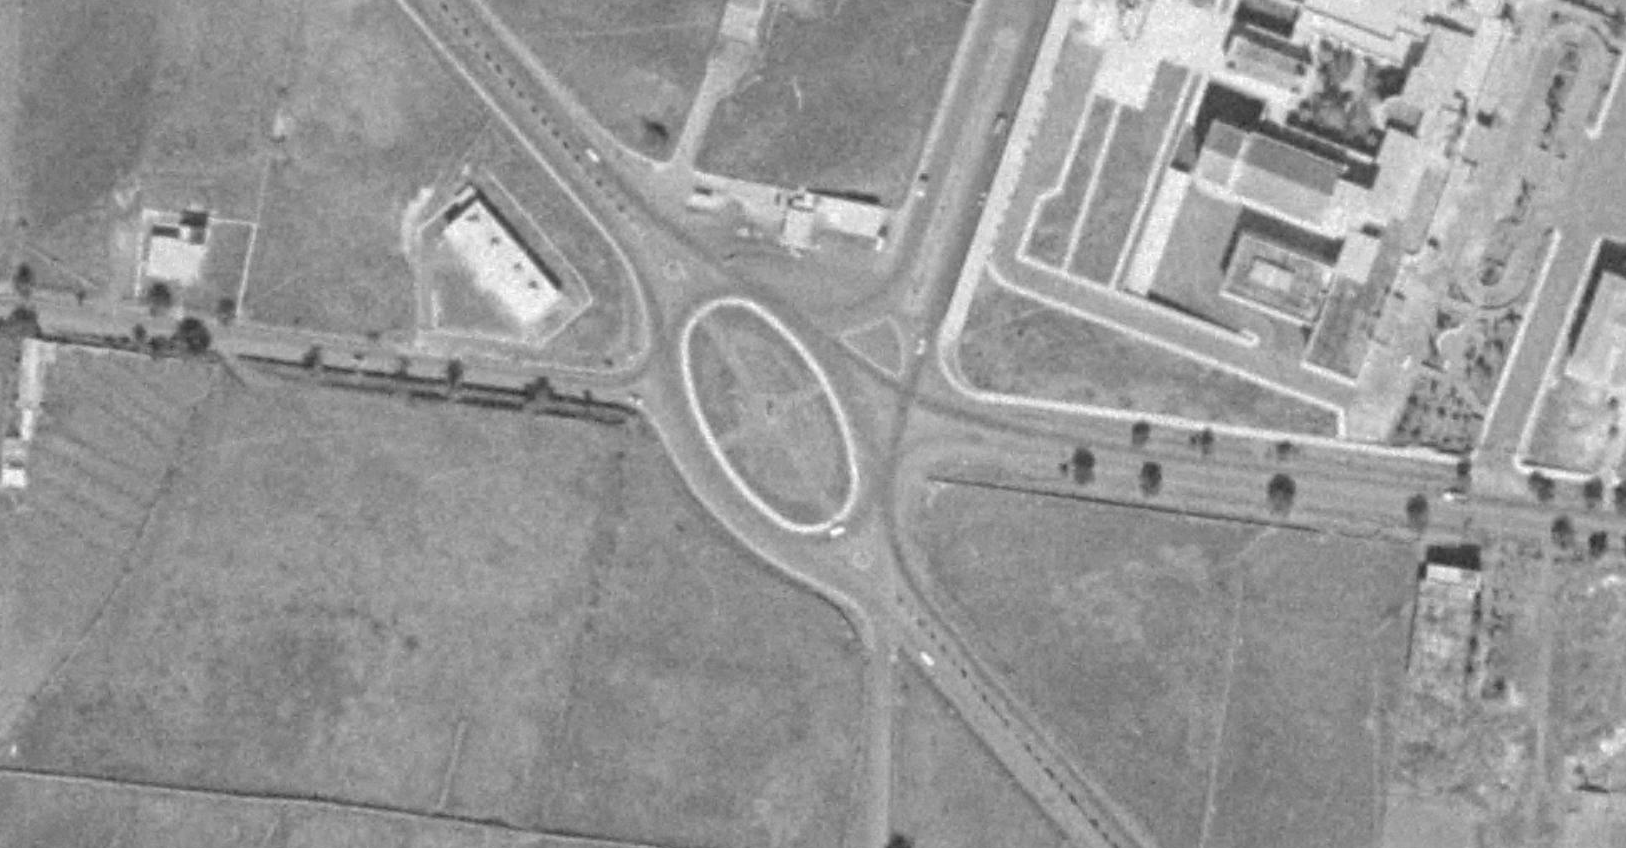
\includegraphics[width=\textwidth]{report/images/amp-anchieta-1964.png}
      \caption{1964}
      \label{fig:anchieta1964}
    \end{subfigure}
    \hfill
    \begin{subfigure}[t]{.49\textwidth}
      \centering
      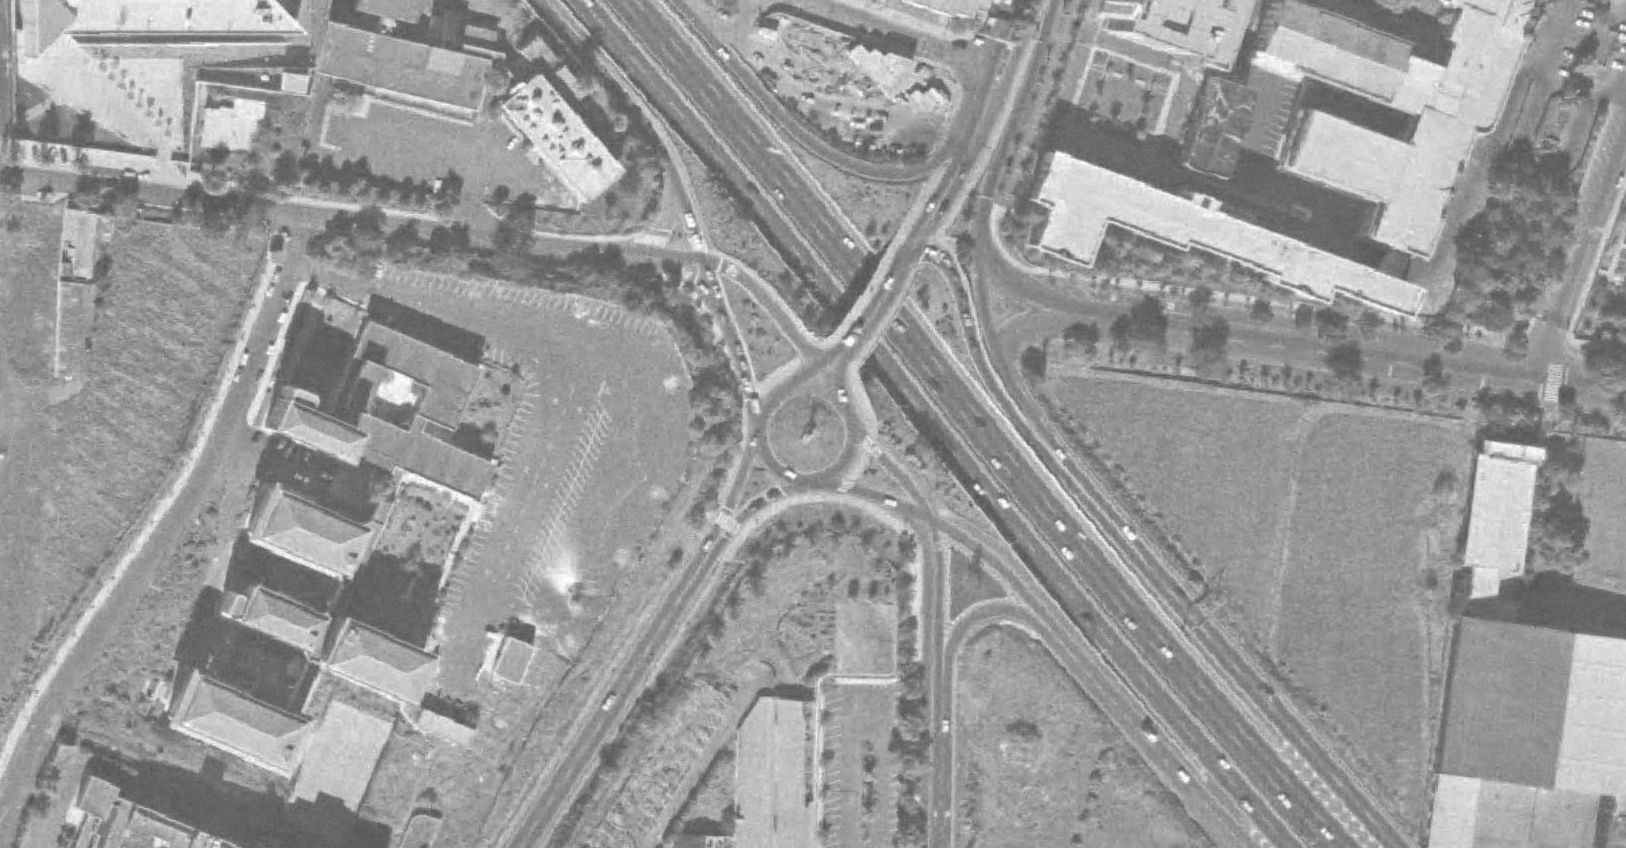
\includegraphics[width=\textwidth]{report/images/amp-anchieta-1994.png}
      \caption{1994}
      \label{fig:anchieta1994}
    \end{subfigure}
    \vspace{0.7cm}
    \begin{subfigure}[t]{.49\textwidth}
      \centering
      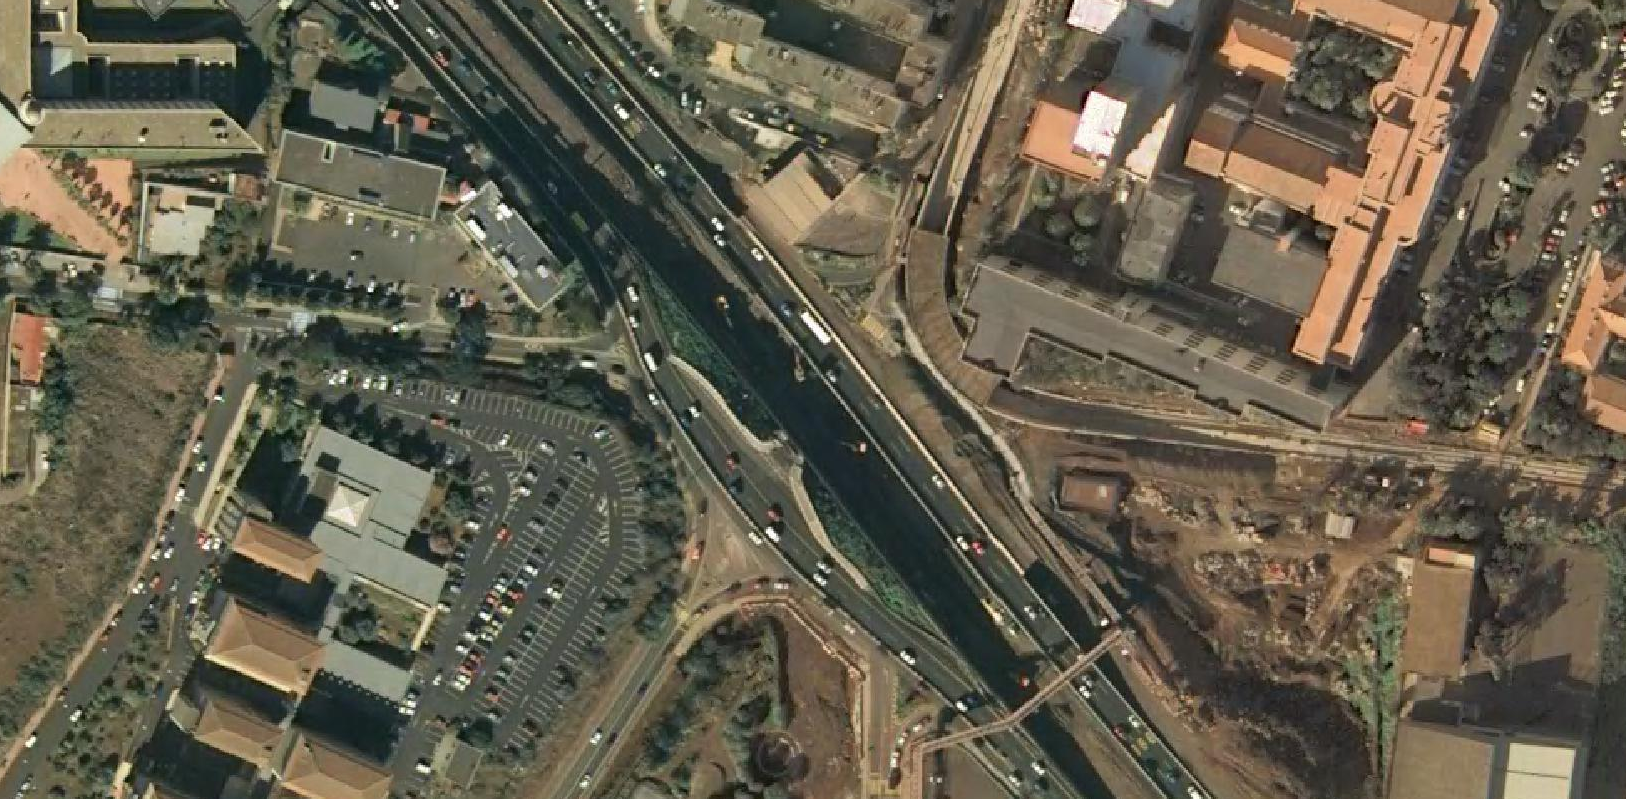
\includegraphics[width=\textwidth]{report/images/amp-anchieta-2006.png}
      \caption{2006 (en obras)}
      \label{fig:anchieta2006}
    \end{subfigure}
    \hfill
    \begin{subfigure}[t]{.49\textwidth}
      \centering
      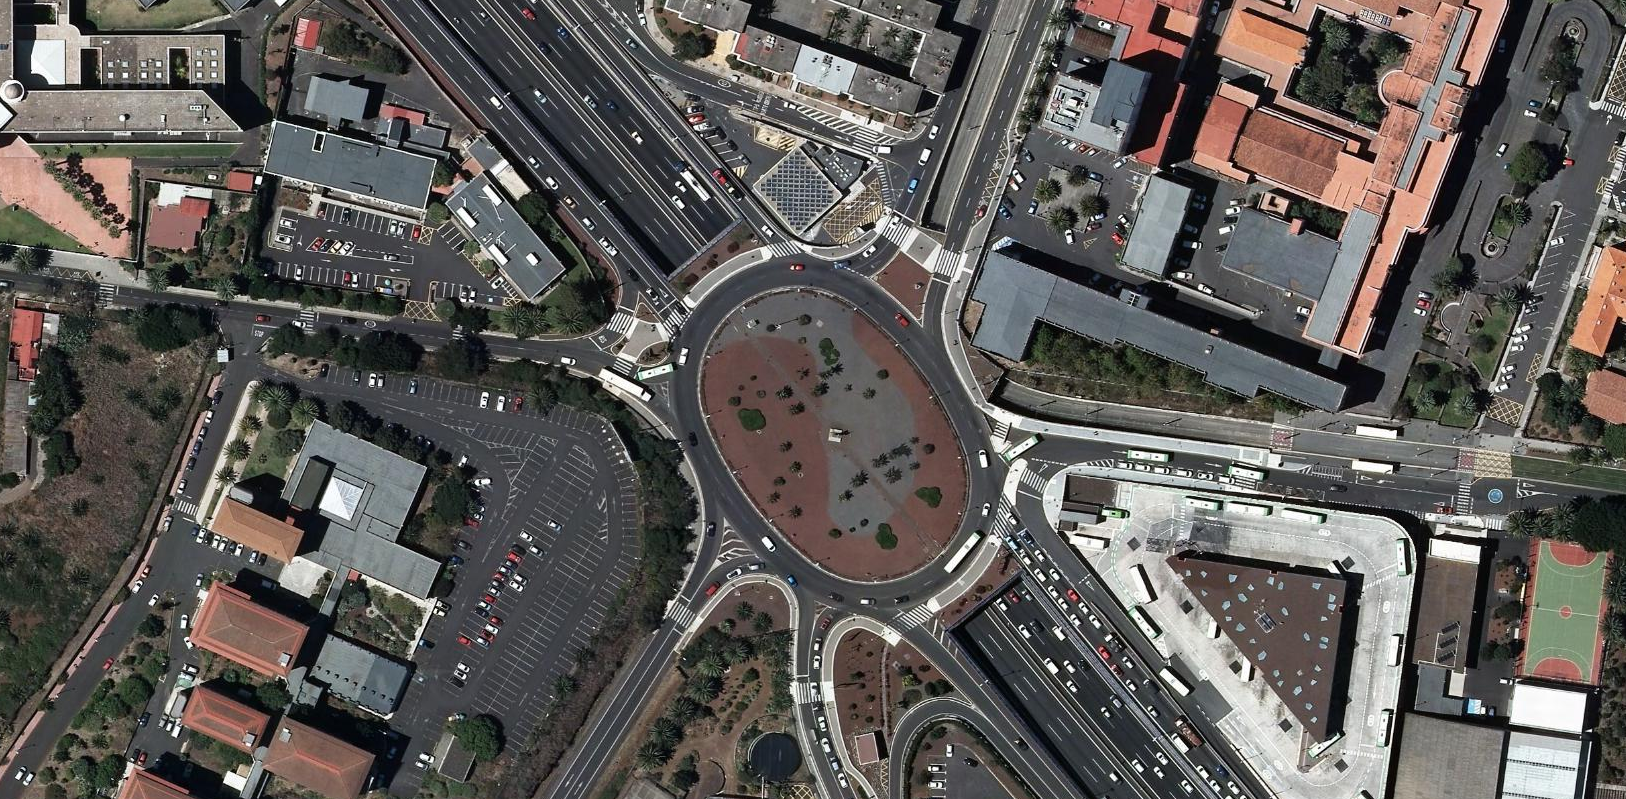
\includegraphics[width=\textwidth]{report/images/amp-anchieta-2019.png}
      \caption{2019}
      \label{fig:anchieta2019}
    \end{subfigure}
    \caption{Evolución de la rotonda de Padre Anchieta a lo largo de los años. Fotografías cortesía de GRAFCAN (\url{https://visor.grafcan.es/visorweb/})}
    \label{fig:anchieta_ev}
\end{figure}

\subsection{Mejoras propuestas}

Las autoridades de la isla no son ajenas al problema de tráfico que plantea de la rotonda. El Cabildo de Tenerife, organismo de cuya competencia depende la rotonda, y el Gobierno de Canarias, de cuya competencia depende la TF-5, han planteado varias medidas, de entre las cuales cabe mencionar:

\begin{itemize}
    \item El soterramiento de la TF-24 en dirección hacia Santa Cruz (a la espera de ejecutar el proyecto)~\cite{dia_cabildo_2019}.
    \item La construcción de una pasarela de peatones sobre la rotonda~\cite{rozas_pasarela_2019}.
    \item Potenciación del vehículo compartido y el transporte público: creación de carriles BUS-VAO en la TF-5~\cite{20minutos_gobierno_2019}.
    \item Propuestas para la construcción de nuevas líneas de tranvía~\cite{redaccion_de_eldiarioes_cabildo_2020}.
\end{itemize}

Sin embargo, todas las medidas mencionadas suponen un cargo importante al erario público, suponen una carga administrativa importante (por todos los procesos de licitación y control que han de realizarse), llevan mucho tiempo construirlas y mientras dure el proceso resultarán un incordio para los conductores y usuarios de la vía.

\section{Objetivos}

Con la elaboración de este proyecto lo que se propone es la instalación de semáforos en la rotonda, cuyas duraciones de fase han sido optimizadas mediante un algoritmo evolutivo, para comprobar si con la instalación de estos semáforos es posible mejorar la circulación del tráfico en función de determinados parámetros como la duración media de los trayectos de los vehículos, la velocidad media, la cantidad de vehículos que han logrado completar su trayecto en una hora, etc.


{\color{BurntOrange} HABLAR DEL TLSP!!!!!}


En comparación con las medidas antes mencionadas, la que se propone supone un coste considerablemente más bajo, no molestaría tanto a los conductores durante la instalación (la cual sería también mucho más corta y sencilla) y que plantea un problema muy interesante que podría ser reaprovechado para otras vías sin coste alguno (si ya tuvieran semáforos instalados).

Para llevar a cabo el proyecto, se han empleado principalmente dos herramientas.

\begin{itemize}
    \item La primera de ellas es SUMO~\cite{lopez_microscopic_2018}, un simulador de tráfico microscópico que nos permitirá evaluar cómo se comporta el tráfico en la rotonda de Padre Anchieta, con datos de tráfico provistos por el Cabildo de Tenerife.
    \item La segunda es Genetics.js~\cite{abrante_dorta_framework_2019}, una librería orientada a algoritmos evolutivos (en particular, algoritmos genéticos) programada en TypeScript.
\end{itemize}

\subsection{Trabajos previos relacionados}

El planteamiento aquí propuesto ya ha sido tratado desde distintas perspectivas por otros autores en los que se basa este TFG, de entre los que cabe resaltar a:

\begin{itemize}
    \item Segredo \textit{et al.}~\cite{segredo_optimising_2019}. El artículo versa sobre el TLSP y el empleo de varios optimizadores mono y multi-objetivos basados en la diversidad, por ser mucho más eficientes y, en consecuencia, ser capaces de lidiar con zonas significativamente más grandes de ciudades como Berlín, París, Estocolmo o Málaga, en vez de unas pocas intersecciones, llegando a simular casi 1000 de estas y más de 2600 vehículos.
    \item Sánchez \textit{et al.}~\cite{sanchez_applying_2008}. El artículo, de 2008, versa también sobre el TLSP pero aplicado a las Ramblas, en Santa Cruz de Tenerife. El autor, con la optimización propuesta de las duraciones de las fases de los semáforos, consigue mejoras notables en la circulación del tráfico.
    \item Dorta Acosta~\cite{dorta_acosta_simulacion_2019}. En este caso se trata de un TFG de un compañero de la Escuela, que versa sobre la instalación de semáforos inteligentes en la rotonda de Padre Anchieta.
\end{itemize}


{\color{BurntOrange} COMPLETAR CON ALGO MÁS? QUIZÁS PONER EN OTRO LUGAR ESTE APARTADO?}











\chapter{Desarrollo del proyecto: definición de los archivos de red y tráfico, simulación y optimización de la circulación}
\label{cap:3-desarrollo}

\section{Definición de la zona de simulación: el archivo de red}
\label{def_zona_sim_archivo_red}

\subsection{Generación y conversión}
\label{gen_conv}

La zona de la rotonda del Padre Anchieta ha sido extraída de \textit{OpenStreetMap} (OSM), servicio gracias al cual ha sido posible obtener una representación fiel y bastante completa de la rotonda y las vías conexas. OSM permite seleccionar una zona del mapa y descargarla en formato \texttt{.osm}.

Aunque inicialmente se había seleccionado una zona considerable grande de la rotonda (incluyendo, por ejemplo, calles de la zona de la Av. Trinidad, como la Obispo Rey Redondo; así como vías de la zona del Coromoto), finalmente se seleccionó una zona que únicamente abarca la rotonda, las entradas y salidas y el tramo de la TF-5 que pasa por debajo, incluyendo las entradas y salidas de la autopista. Esto se debe a que los datos de tráfico disponibles se circunscriben únicamente a las zonas mencionadas, por lo que no se podría haber simulado otras vías conexas sin perder fiabilidad en la simulación (al tener que aproximar los datos de los vehículos que circulan por dichas vías, en vez de contar con datos empíricos).

OSM ofrece los datos en formato <<.osm>>; sin embargo, los archivos de red legibles por SUMO y las demás herramientas del simulador siguen un formato XML con extensión \texttt{.net.xml}. Para realizar la conversión se empleó una de las herramientas que viene con el simulador, denominada \texttt{NETCONVERT}. Esta herramienta está específicamente destinada a importar archivos redes viales de diferentes fuentes para generar redes viales que puedan ser utilizadas por otras herramientas~\cite{noauthor_netconvert_nodate} (como SUMO, NetEdit, etc.).

% El comando empleado para ejecutar \texttt{NETCONVERT} fue el siguiente:

% \begin{lstlisting}[breaklines=true]
% netconvert --type-files osmNetconvert.typ.xml,osmNetconvertPedestrians.typ.xml --osm-files <Archivo OSM> --output-file <Nombre del archivo de salida> --geometry.remove --roundabouts.guess --ramps.guess --junctions.join --tls.guess-signals --tls.discard-simple --tls.join --no-turnarounds.except-deadend --crossings.guess --osm.all-attributes --sidewalks.guess
% \end{lstlisting}

Los archivos \texttt{xml} que se pasan al comando vienen predefinidos en el pack de herramientas de SUMO, y sirven principalmente para definir el modo en que se clasificarán las vías en el momento de convertirlas (por ejemplo, qué vías se clasificarán como calles o autopistas, con qué velocidad, etc.), así como la adición de aceras y pasos peatonales. El resto de \textit{flags} señalan a \texttt{NETCONVERT} cómo debe realizar la conversión (por ejemplo, pidiendo que infiera las intersecciones, los carriles de aceleración y desaceleración de las autopistas, etc.).

El archivo que obtenemos como resultado del proceso de conversión es con el cual podemos empezar a trabajar con SUMO y las herramientas que trae consigo.

\subsection{Limpieza}

\subsubsection{Intersecciones}

Pese a que \texttt{NETCONVERT} hace un excelente trabajo generando el archivo de red, todavía es necesario realizar pequeños cambios antes de que pueda llevarse a cabo la simulación. Esto se realizó mediante \texttt{NETEDIT}, otra de las herramientas que viene en el paquete de SUMO, y que está orientada a editar archivos de red mediante una GUI, ya sea para modificar las vías (o los metadatos de estas), la forma de las intersecciones, los semáforos, el orden de preferencias en las vías, y toda una serie de funcionalidades relacionadas~\cite{noauthor_netedit_nodate}. El trabajo principal que se ha realizado en este aspecto tiene que ver con la forma de las intersecciones. 

La manera en que dos vías se conectan en SUMO (y, por extensión, en \texttt{NETEDIT}) viene determinada por el Modelo de Intersección de Vías de SUMO~\cite{erdmann_sumos_2014}. Explicado superficialmente, en SUMO la red de vías se representa mediante un grafo. Una intersección consiste en un nodo \textit{de entrada} y otro \textit{de salida} (donde un nodo representa una vía con un identificador concreto, y que sea de entrada o de salida implica de dónde viene y hacia donde va un vehículo). Así pues, un carril de entrada puede tener varios carriles de salida posibles (o sea, varios destinos que puede tomar un vehículo en una intersección).

Bien, dentro de esta intersección existen los denominados <<carriles internos>>, que conectan los nodos de entrada con los de salida y permiten especificar con exactitud por donde deben circular los vehículos en la intersección. Estos carriles internos son calculados automáticamente por \texttt{NETCONVERT}, pero a veces falla o los calcula de una manera inexacta, lo que provoca que algunas intersecciones proporcionadas por el conversor no representen con fidelidad la  intersección real.

Asimismo, es muy importante configurar bien las intersecciones puesto que son necesarias para añadir los semáforos y configurarlos adecuadamente en función de las vías que vaya a regular; situación que también se da para los pasos de peatones.

La mayoría del trabajo de limpieza consistió, pues, en procurar la exactitud de las intersecciones de las vías de entrada y salida de la rotonda. Esto es posible modificando la forma de estas en \texttt{NETEDIT}; pero, por desgracia, es un trabajo en gran parte tedioso y a veces frustrante, puesto que la manera en que están definidas estas intersecciones es mediante un conjunto de puntos (que encierran la zona por la que pasan los carriles internos, como se ve en la figura~\ref{fig:interseccion3}). 

\begin{figure}[ht]
    \centering
    \begin{subfigure}[t]{.30\textwidth}
      \centering
      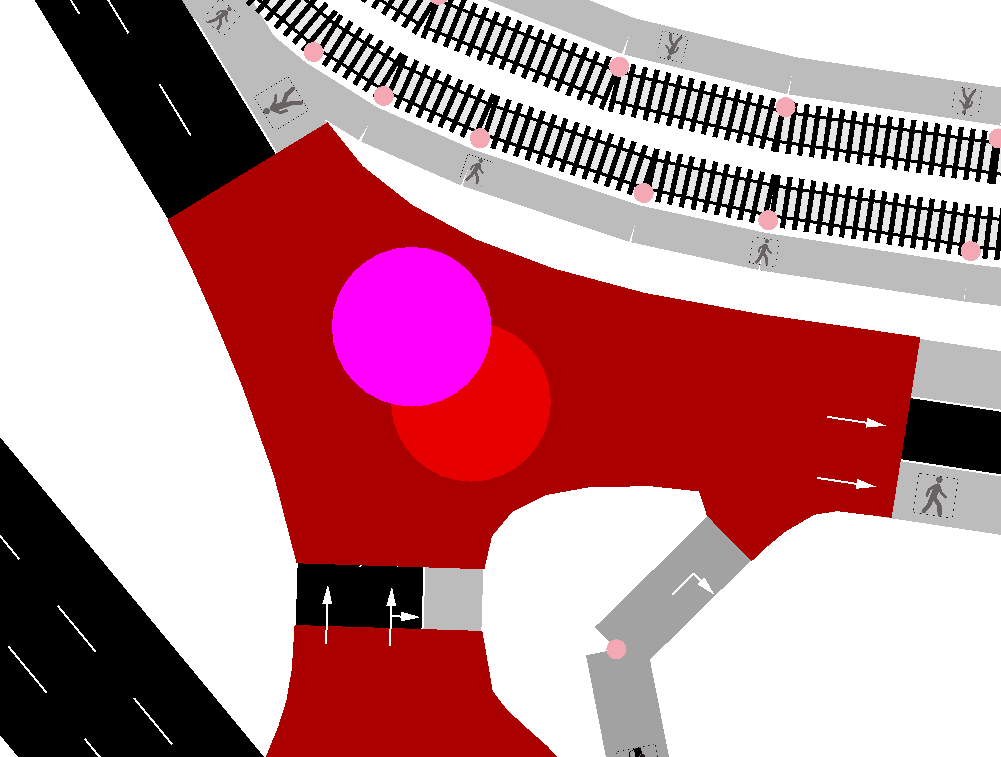
\includegraphics[width=\textwidth]{report/images/interseccion1.png}
      \caption{Forma de la intersección (señalada en rojo).}
      \label{fig:interseccion1}
    \end{subfigure}
    \hfill
    \begin{subfigure}[t]{.30\textwidth}
      \centering
      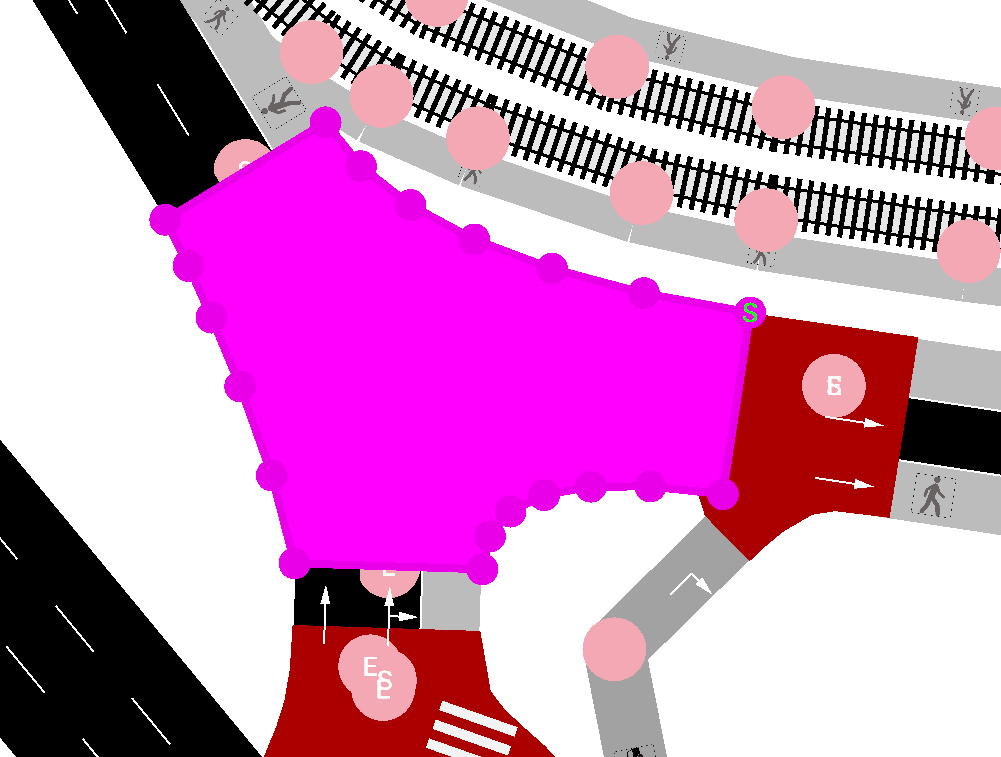
\includegraphics[width=\textwidth]{report/images/interseccion2.png}
      \caption{Modo de edición de la intersección (en violeta). Se aprecian los puntos que definen la forma.}
      \label{fig:interseccion2}
    \end{subfigure}%
    \hfill
    \begin{subfigure}[t]{.30\textwidth}
      \centering
      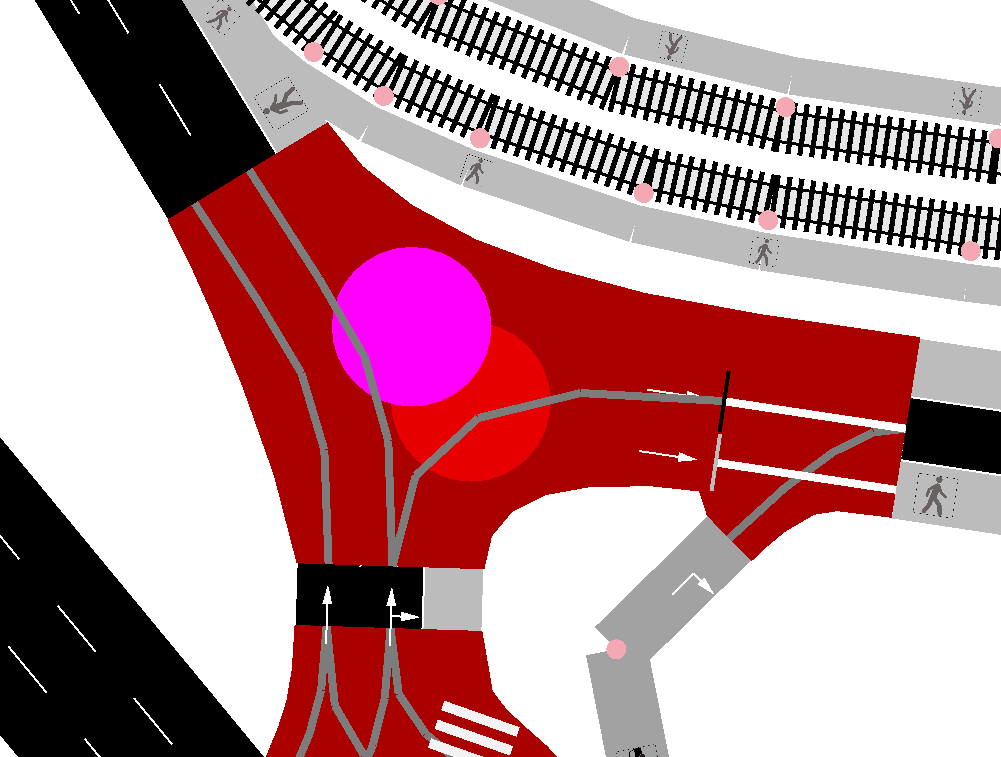
\includegraphics[width=\textwidth]{report/images/interseccion3.png}
      \caption{Carriles internos (señalados en gris). La forma de estos depende de la forma de la intersección.}
      \label{fig:interseccion3}
    \end{subfigure}
    \caption{Representación de las intersecciones en \texttt{NETEDIT}.}
    \label{fig:interseccion}
\end{figure}

Además, cabe mencionar que \texttt{NETEDIT}, en determinadas circunstancias o al intentar algunas modificaciones en concreto, ha llegado a cerrarse de forma inesperada debido a un error interno del programa, resultando además que se perdía todo el trabajo realizado hasta el momento, por lo que había que empezar de nuevo.

\subsubsection{Vías mal priorizadas}

Para señalar la prioridad de una vía sobre otra, SUMO asigna un \textit{valor de prioridad} en función del tipo de vía que sea, de acuerdo con una clasificación que también emplea \textit{OpenStreetMap}. Por ejemplo, una autopista tiene prioridad sobre las carreteras primarias, estas sobre las carreteras secundarias, estas sobre las calles urbanas, etc. 

Durante el proceso de conversión es posible que algunas vías no estén señaladas o priorizadas adecuadamente, dando lugar a que los ceda el paso se produzcan por vías a las que en realidad les corresponde la prioridad en una intersección. Este fue el caso de algunas entradas de la rotonda.

Hay una \textit{flag} que se puede añadir al comando \texttt{NETCONVERT} mencionado en la sección~\ref{gen_conv} que se denomina \texttt{--roundabouts.guess}. Esta \textit{flag} permite que, durante el proceso de conversión, se detecten automáticamente las rotondas y se ajusten las prioridades de acuerdo con la norma general: las vías de la rotonda en sí tienen prioridad sobre las vías de entrada. Sin embargo, al ser un método heurístico, es posible que falle y es el caso ante el cual nos encontramos.

Por suerte, corregirlo no es particularmente complicado. Basta con reducir el valor de prioridad de la vía de entrada con respecto al de la rotonda y problema solucionado.

\subsubsection{Vías mal representadas}

Este es un caso bastante particular y tiene que ver con la salida de la TF-5, en dirección norte, que permite incorporarse a la rotonda de Padre Anchieta (representado en la figura \ref{fig:salida-tf5-norte}). 

\begin{figure}[ht]
    \centering
    \begin{subfigure}[t]{0.48\textwidth}
      \centering
      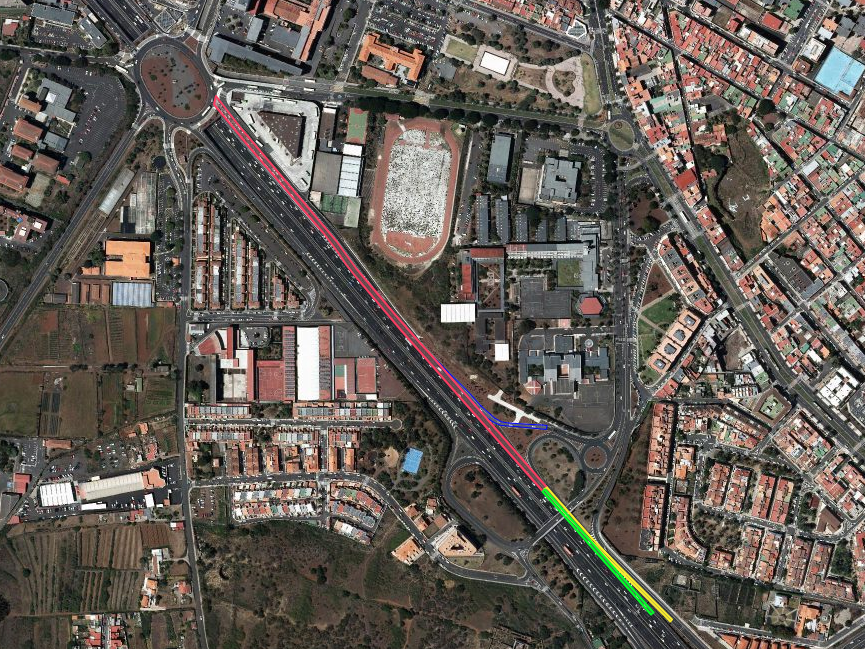
\includegraphics[width=\textwidth]{report/images/salida-tf5-norte-lejos_.png}
      \caption{La salida de la TF-5 (dir. norte) a la rotonda de Padre Anchieta vista desde lejos.}
      \label{fig:salida-tf5-norte-lejos}
    \end{subfigure}
    \hfill
    \begin{subfigure}[t]{0.48\textwidth}
      \centering
      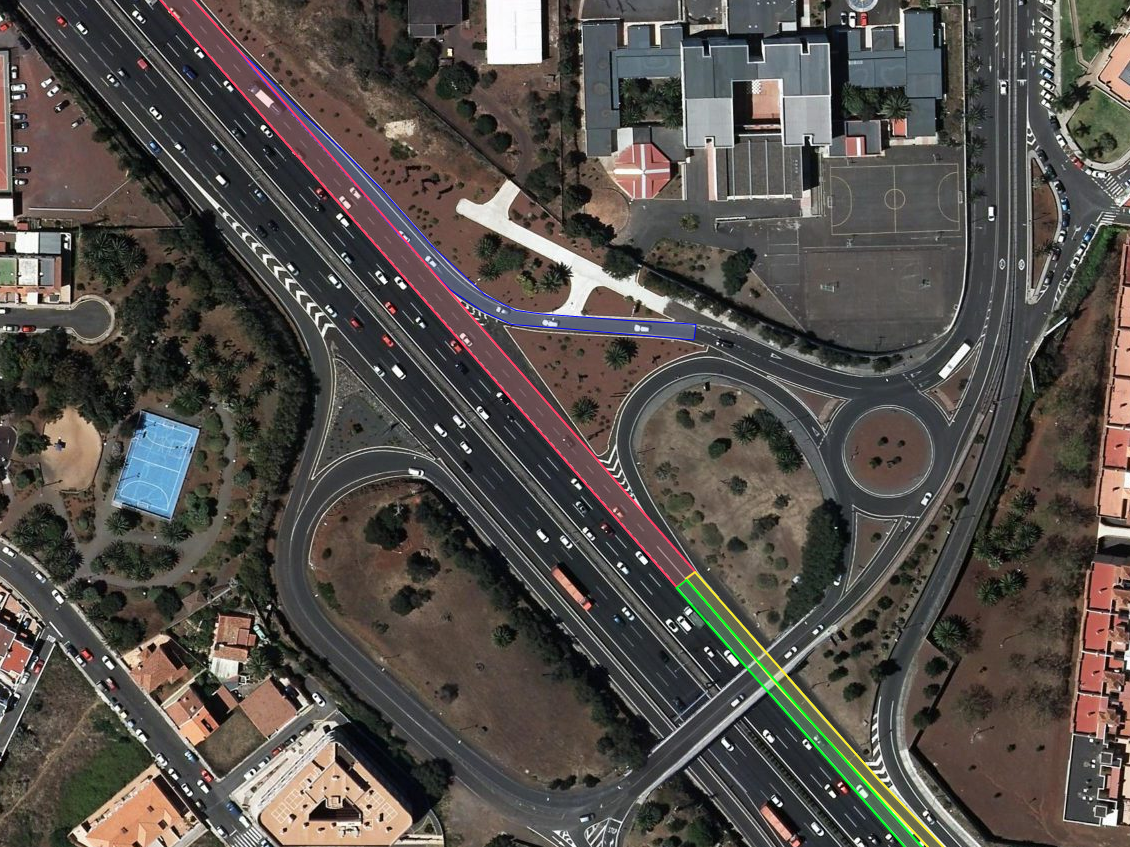
\includegraphics[width=\textwidth]{report/images/salida-tf5-norte-cerca_.png}
      \caption{La misma vista, desde cerca. Permite apreciar los distintos carriles que dan lugar o se incorporan a la salida en cuestión.}
      \label{fig:salida-tf5-norte-cerca}
    \end{subfigure}%
    \caption{La zona roja representa la vía de doble carril (el de la izquierda permite la incorporación a la autopista y también ir a la rotonda de Padre Anchieta, mientras que el derecho permite ir a la rotonda únicamente). La azul se corresponde con la carretera proveniente del IES Viera y Clavijo. El carril verde es el proveniente de la autopista, y el amarillo el proveniente de la rotonda que está por debajo de la autopista. Los tres dan lugar a la vía representada por la zona roja.}
    \label{fig:salida-tf5-norte}
\end{figure}

Bien, la vía representada zona roja (figura~\ref{fig:salida-tf5-norte-cerca}) permite ir a la rotonda o incorporarse a la autopista. Esta incorporación a la TF-5 tiene sentido para los vehículos que vienen de la zona azul o la amarilla. También tendría sentido para los vehículos que provinieran de la autopista (zona verde) que pese a haber tomado la salida deseen reincorporarse a la autopista.

Este comportamiento es el correcto; sin embargo, durante el proceso de conversión \texttt{NETCONVERT} se equivocó y generó un archivo de red que no permitía que los vehículos provenientes de las zonas mencionadas pudieran incorporarse a la TF-5 en dicho lugar (figura~\ref{fig:netedit-tf5-norte-mal}), lo que provocaba que tuvieran que pasar por la rotonda de Padre Anchieta y tomar desde ahí la salida en dirección a la TF-5. Tal comportamiento es indeseable y se corrigió.

\begin{figure}[ht]
    \centering
    \begin{subfigure}[t]{0.48\textwidth}
      \centering
      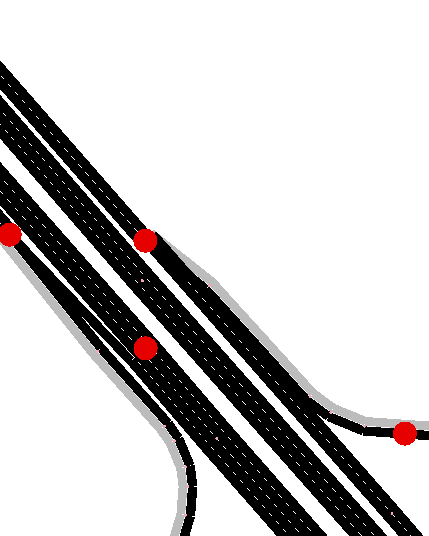
\includegraphics[width=\textwidth]{report/images/netedit-tf5-norte-mal.png}
      \caption{Generación inicial. Véase cómo no es posible la incorporación a la autopista desde los dos carriles que aparecen más a la derecha, que separados de los tres que están en medio (TF-5 dirección norte).}
      \label{fig:netedit-tf5-norte-mal}
    \end{subfigure}
    \hfill
    \begin{subfigure}[t]{0.48\textwidth}
      \centering
      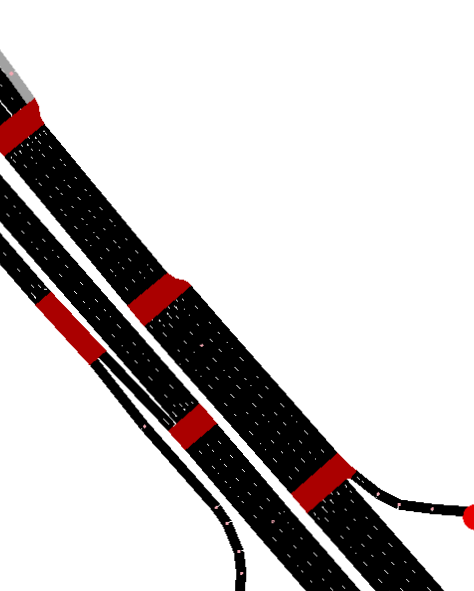
\includegraphics[width=\textwidth]{report/images/netedit.-tf5-norte-bien.png}
      \caption{Modificación realizada. Ahora los vehículos pueden incorporarse a la autopista, pero también los de la autopista pueden tomar la salida más adelante de lo que deberían.}
      \label{fig:netedit-tf5-norte-bien}
    \end{subfigure}%
    \caption{Cambios realizados en la salida de la TF-5 (dir. norte) que va a la rotonda del Padre Anchieta.}
    \label{fig:netedit-tf5-problema}
\end{figure}

Sin embargo, por limitaciones de SUMO, actualmente no es posible establecer carriles con prohibición de cambio asimétrica (como es el caso de la zona roja que se menciona antes): es decir, actualmente no se puede implementar un cambio de carril de modo que sea posible incorporarse a la autopista pero no sea posible realizar la acción inversa. Ello implica que con la modificación realizada para solucionar el problema los vehículos que vayan por la autopista podrán tomar la salida mucho más adelante de lo que en realidad pueden hacerlo (figura~\ref{fig:netedit-tf5-norte-bien}). No obstante, esta solución, aunque imperfecta, es mejor que impedir la incorporación a la TF-5 por los motivos mencionados en el párrafo anterior.

\subsubsection{Otras modificaciones}

Mencionadas las modificaciones más sustanciales, en el archivo de red también se han realizado otras modificaciones menores como la forma de algunas vías (especialmente las vías de la rotonda en sí), que han sido retocadas para que sean más fieles a la realidad; la adición de pasos de peatones, la adición de aceras cuando era necesario y la supresión cuando eran aceras innecesarias o no se correspondían con la realidad, la configuración de los semáforos (de la que se hablará en su propia sección), la corrección de algunas conexiones que permitían giros prohibidos, etc.

\section{Definición de los vehículos y las rutas: el archivo de tráfico}

El principal objetivo a la hora de generar el tráfico y los peatones era hacerlo para una hora de simulación, de modo que dicha hora fuera punta (por ejemplo, a las 8:00 o las 14:00).

En este sentido, varios enfoques han sido tomados en cuenta, resultando al final como ganador la generación de tráfico en función de un algoritmo de maximización del flujo de red, con datos empíricos de aforadores de tráfico provistos por el Cabildo de Tenerife, gracias a un estudio que realizó la entidad en noviembre de 2019 en la rotonda de Padre Anchieta. 

Sin embargo, es relevante mencionar otros enfoques que en durante el desarrollo de este proyecto se tomaron en cuenta, dado que los datos del Cabildo se obtuvieron más adelante durante la fase de desarrollo de este trabajo.

\subsection{Enfoque estocástico}

Este enfoque es el más sencillo. Consiste en generar los datos de tráfico y de peatones de forma aleatoria, tanto en flujo como en rutas. SUMO cuenta con una herramienta para hace precisamente esto, \texttt{randomTrips.py}~\cite{noauthor_randomtripspy_nodate}, un script de Python que, con un archivo de red como entrada, permite generar sendos archivos de tráfico y peatones aleatorios.

Las desventajas que plantea este método saltan a la vista: los datos de tráfico generados muy probablemente no se correspondan con la realidad. Esto plantea un problema serio a la hora de obtener una simulación fiel, puesto que los datos de circulación en una situación como la actual pueden afectar sensiblemente al resultado final de la simulación y, en consecuencia, no se podría determinar con fiabilidad si los semáforos son una adición útil o no (que al final es el objetivo último de este trabajo).

A falta de datos de tráfico, este enfoque parece el más aceptable. Sin embargo, el Cabildo de Tenerife publica anualmente un estudio de las intensidades de tráfico en las carreteras de Tenerife~\cite{rodriguez_hernandez_intensidades_2019}. Este estudio no contiene los datos de los aforadores de la rotonda de Padre Anchieta que se mencionaban antes, pero sí contiene la intensidad media diaria (IMD) anual de algunas vías que conectan con la rotonda. La IMD anual de define como el número de vehículos que pasan a través de una sección fija de la carretera dividido entre 365.

Por ejemplo, de las vías que nos interesan el informe contiene los datos de la IMD anual de la TF-5, de la TF-24 (la carretera de La Esperanza) y de la TF-263 (la carretera de Geneto). También tienen datos de la TF-265 (Camino de San Francisco de Paula) pero dicha carretera no conecta directamente con la rotonda, sino que lo hace con la Av. Astrofísico Francisco Sánchez, que sí es una vía de que entra y sale de la rotonda.

Estos datos son extremadamente débiles para inferir el tráfico en una hora particular, sobre todo si queremos el caso de la hora punta de las vías en cuestión. Y eso sin mencionar de que todavía nos faltarían datos de otras vías. Ello nos lleva a plantear el siguiente método.

Sin embargo, este sí fue el enfoque empleado para generar los peatones, puesto que no se dispone de ningún dato sobre los movimientos de las personas que atraviesan los pasos de peatones de las vías conexas de la rotonda.


\subsection{Enfoque de inundación}


\begin{wrapfigure}{L}{5.5cm}
    \centering
    % \captionsetup{width=.8\linewidth}
    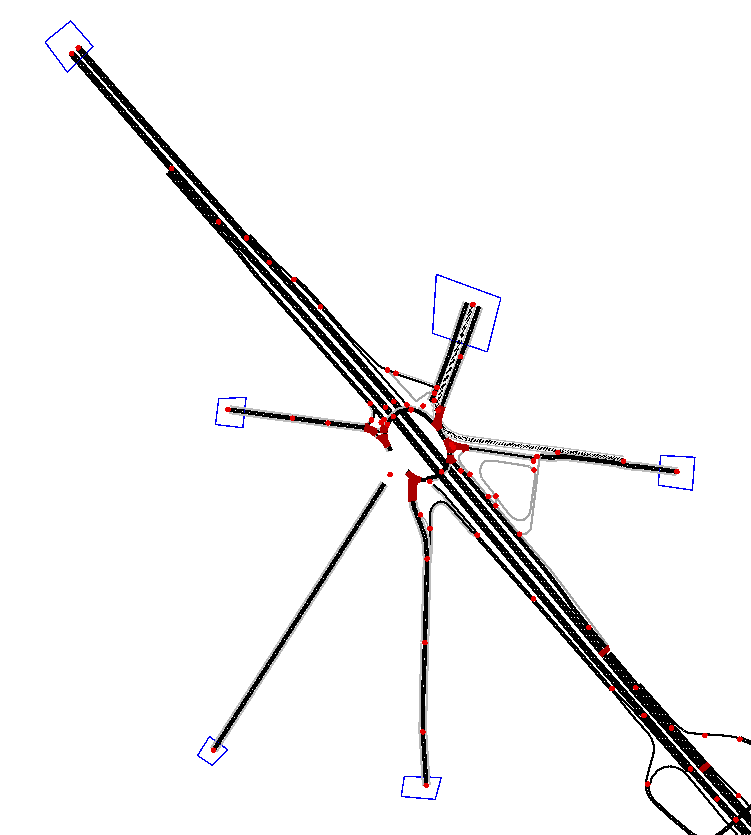
\includegraphics[width=\linewidth]{report/images/taz.png}
    \caption{Las TAZ aparecen delimitadas por las líneas azules.}
    \label{fig:taz}
\end{wrapfigure}


A falta de datos para generar el tráfico, un enfoque interesante residía en generar el tráfico de modo que se lleva al límite el aforo de las vías de la rotonda; es decir, propiciando que circulara el máximo tráfico posible por todas las vías. Este enfoque, aunque en determinados casos resulte irreal, en cierta medida no es tan diferente de lo que sucede en realidad, puesto que en horas punta la rotonda de Padre Anchieta sufre de colas en todas las entradas (en las entradas desde autopista, tanto del norte como del sur, en la Av. Trinidad, en la carretera de la Esperanza y la de Geneto).

Una manera de definir el archivo de tráfico de este enfoque es mediante matrices origen-destino (\textit{O/D matrices})~\cite{otto_anker_nielsen_two_1998}, las cuales se centran en definir el lugar de partida y de llegada junto con el flujo (cantidad de vehículos que circularán desde A hasta B).

Dado que nuestro archivo de red es lo suficientemente pequeño, es viable definir todos los posibles orígenes y destinos de nuestras rutas, asignando un flujo a cada una de ellas lo suficientemente alto como para que pueda haber circulación de vehículos durante una hora.

SUMO viene preparado con una herramienta (\texttt{OD2TRIPS}~\cite{noauthor_od2trips_nodate}) que puede leer archivos de matrices O/D en un formato concreto y convertirlos al formato de archivo de tráfico que nos interesa para realizar la simulación.

La manera en que se definen las matrices O/D viene especificada en~\cite{noauthor_demandimporting_nodate}. La definición de los orígenes se realiza mediante TAZ (\textit{Traffic Analysis Zone}), zonas que se señalan en el archivo de red para agrupar un conjunto de vías de forma que sea fácil establecer el nodo donde se debe iniciar el trayecto y el nodo donde debe finalizar (véase la figura~\ref{fig:taz}).

Este enfoque, como se mencionó antes, solo resultaría útil hasta cierto punto, puesto que solamente representa un estado particular de la rotonda. Generalmente, la rotonda no absorbe el máximo aforo posible en todas las vías, por lo que un enfoque más preciso sería conveniente.

\subsection{Enfoque empírico}

Este enfoque es el que al final se ha empleado, puesto que transcurrido cierto tiempo desde el inicio del proyecto fue posible obtener datos de tráfico correspondientes a 21 aforadores colocados en las inmediaciones de la rotonda, en un estudio realizado por el Cabildo de Tenerife en la semana del 19 al 25 de noviembre de 2019 (véase la figura~\ref{fig:aforadores}). Estos datos vienen desglosados por aforador, día y hora. Los datos de la autopista se obtuvieron desde la web (también del Cabildo) \url{http://154.48.153.16:8080/aforos/}.

\begin{figure}[ht]
    \centering
    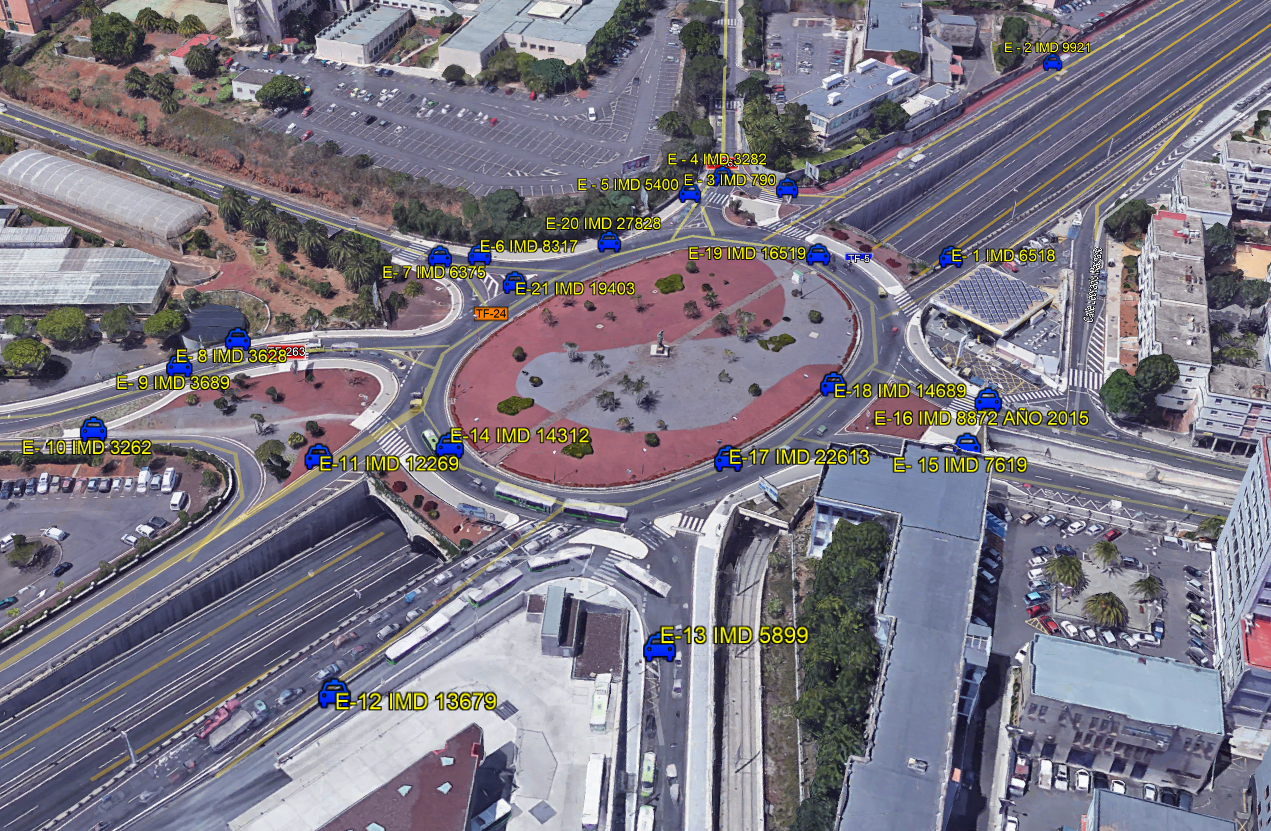
\includegraphics[width=\textwidth]{report/images/aforadores.png}
    \caption{Lugares donde se instalaron los aforadores.}
    \label{fig:aforadores}
\end{figure}

Como nuestro objetivo era simular una hora punta, nos acabamos decantando por obtener los datos del día jueves 21 de noviembre de 2019, a las 8:00, por ser el día que más tráfico hubo a esa hora.

\subsubsection{Generación de rutas: \texttt{flowrouter.py}}

Tener los datos de los aforadores es una gran ayuda a la hora de estimar con fiabilidad el tráfico real de la rotonda, pero no lo es todo, puesto que no indica qué ruta han seguido dichos vehículos ni tampoco cuál es el destino al que habían de llegar. Es decir, es conocido cuántos coches salen de A y cuántos llegan a B, pero no conocemos cuáles de los coches que han llegado a B procedían de A. Al final, de lo que disponemos es de contadores de vehículos, pero lo que nos interesa son las rutas que siguen dichos vehículos; o sea, una matriz O/D.

Así pues, el problema de inferir una matriz O/D a partir de datos de contadores de tráfico no es en absoluto desconocido y abunda bastante literatura sobre cómo abordar este problema (véase~\cite{otto_anker_nielsen_two_1998}). 

Sin embargo, y como no podía ser de otro modo, los creadores de SUMO ya habían previsto que esta situación podría darse, así que decidieron incorporar dos herramientas para calcular las rutas con sus respectivos flujos a partir de datos de aforadores: \texttt{DFROUTER}~\cite{noauthor_dfrouter_nodate}; y su versión mejorada, \texttt{flowrouter.py}~\cite{noauthor_flowrouterpy_nodate,behrisch_route_2018}, la cual ha sido finalmente la empleada para generar el tráfico.

La diferencia entre ambas radica en el algoritmo que emplean para calcular las rutas y los flujos de los vehículos. \texttt{DFROUTER} está pensada para redes en las cuales todas las posibles entradas y salidas cuentan con aforadores, y los datos que estos brindan son relativamente precisos. \texttt{flowrouter.py}, por otro lado, está pensado para trabajar con más incertidumbre y, por tanto, es capaz de lidiar con redes en las cuales faltan aforadores y donde los datos pueden presentar cierto nivel de inconsistencia.

Estas herramientas toman como entrada tres archivos:

\begin{itemize}
    \item El archivo de red.
    \item Un archivo con los datos de los aforadores (nombre, posición, y si es de origen, destino o está <<en medio>> ---esta clasificación, tal y como se infiere de su nombre, está reservada para aforadores que no son clasificables como de origen o destino---).
    \item Datos de flujo (aforador, flujo, plazo durante el cuál se detectó dicho flujo, etc.).
\end{itemize}

Y como salida general dos archivos:

\begin{itemize}
    \item Un archivo de rutas.
    \item Un archivo de flujos (definidos en función de las rutas).
\end{itemize}

Ha de señalarse que ambas herramientas están pensadas para trabajar con redes relativamente simples, concretamente autopistas, dado que suelen estar bien dotadas de aforadores y no poseen una topología especialmente compleja; por lo que es posible que los resultados que brindan dichas herramientas a veces pueden ser erráticos y confusos, por lo que la entrada debe ser lo más completa y precisa posible.

Durante una prueba inicial, los resultados obtenidos con \texttt{flowrouter.py} mostraban que había rutas que no seguía ningún vehículo cuando realmente debía de haber algún flujo. También, en algunos casos, se generaban rutas ilógicas, como circular desde la carretera de Geneto con la intención de incorporarse a la TF-5 sentido sur pasando por la rotonda, ignorando el desvío (más corto) del que dispone la carretera, que permite incorporarse a la autopista directamente.

Es muy posible que este tipo de errores e inexactitudes se produjeran por la intención del algoritmo de satisfacer las restricciones impuestas por los datos de los aforadores. Asimismo, la configuración de algunos de estos contadores no era la idónea. 

Por ejemplo, volviendo al caso de la carretera de Geneto, según muestra la figura~\ref{fig:aforadores}, esta cuenta con tres aforadores: el E-8 (en sentido ascendente), el E-9 (en sentido descendente) y el E-10 (en sentido descendente, colocado en el desvío hacia la autopista).

Se da la circunstancia de que, por la manera en que \texttt{flowrouter.py} calcula las rutas, es posible que designara los orígenes y los destinos en unos nodos en los cuales realmente no deseamos que acabe el tráfico (porque, por ejemplo, no daría tiempo a que se formaran colas o a apreciar mejor durante la simulación el funcionamiento del tráfico).

Todos estos problemas se solucionaron (en su mayoría) añadiendo nuevos contadores manualmente. Para el ejemplo que estamos tratando, bastó con añadir un contador en la carretera de Geneto, sentido descendente, que estuviera un poco más arriba y que sumara el flujo de los contadores E-9 y E-10, y colocando a la misma altura el contador E-8 (el que estaba en sentido ascendente). Hecho con el resto de vías, la generación del tráfico es menos errática y durante la simulación es posible apreciar mejor el flujo de los vehículos.

Este método es, pues, el que mejor resultados ha brindado y es con el que finalmente se llevó a cabo la generación del tráfico.

\section{Los semáforos de la rotonda: configuraciones}

Una vez definidos el archivo de red y el de tráfico, llega el momento de tomar una decisión importante: ¿dónde han de situarse los semáforos? A fin de cuentas, la rotonda de Padre Anchieta no es una zona que contara previamente con semáforos, por lo que nos corresponde a nosotros determinar la localización de estos.

Así pues, se proponen tres configuraciones distintas:

\paragraph{Configuración 1: Semáforos en cada entrada y salida, con el carril interior siempre en verde.}

Una posible configuración de los semáforos es añadir uno en cada entrada y salida de la rotonda, de modo que esté absolutamente regulada por estos. Además, el carril interior permanecería en verde siempre que fuera posible, cambiando de color únicamente en los casos en los que la vía entrada a la rotonda tenga dos carriles y sea necesario regular el paso entre los carriles izquierdos de la entrada y la rotonda. 

\paragraph{Configuración 2: Semáforos en cada entrada y salida, con el carril interior cambiando de color.} Es la misma configuración que la 1, con la salvedad de que el carril interior cambia de color junto con el exterior independientemente de que la entrada que se esté regulando tenga un carril o dos. El objetivo de simular estas dos configuraciones es comprobar cuál es más eficiente gestionando el carril interior. Véase la figura~\ref{fig:conf2}. Tanto en esta configuración como en la anterior, las fases se modificaron manualmente para garantizar que siguen un ciclo correcto.

\paragraph{Configuración 3: Semáforos al norte y al sur de la rotonda.} Este caso particular solamente instala dos semáforos: uno al norte de la rotonda (entre la entrada de la TF-5 en sentido Santa Cruz y la salida hacia la TF-5 en sentido La Orotava) y otro al sur (entre la salida hacia la TF-5 en sentido Santa Cruz y la entrada de doble carril desde la TF-5 en sentido La Orotava). Véase la figura~\ref{fig:conf3}. Esta configuración permitiría partir la rotonda a la mitad, en función del tráfico que circula a través de cada una de ellas, con el objetivo de facilitar la circulación. \textcolor{red}{Revisar esta frase.}


\begin{figure}[ht]
    \centering
    \begin{subfigure}[t]{0.48\textwidth}
        \centering
        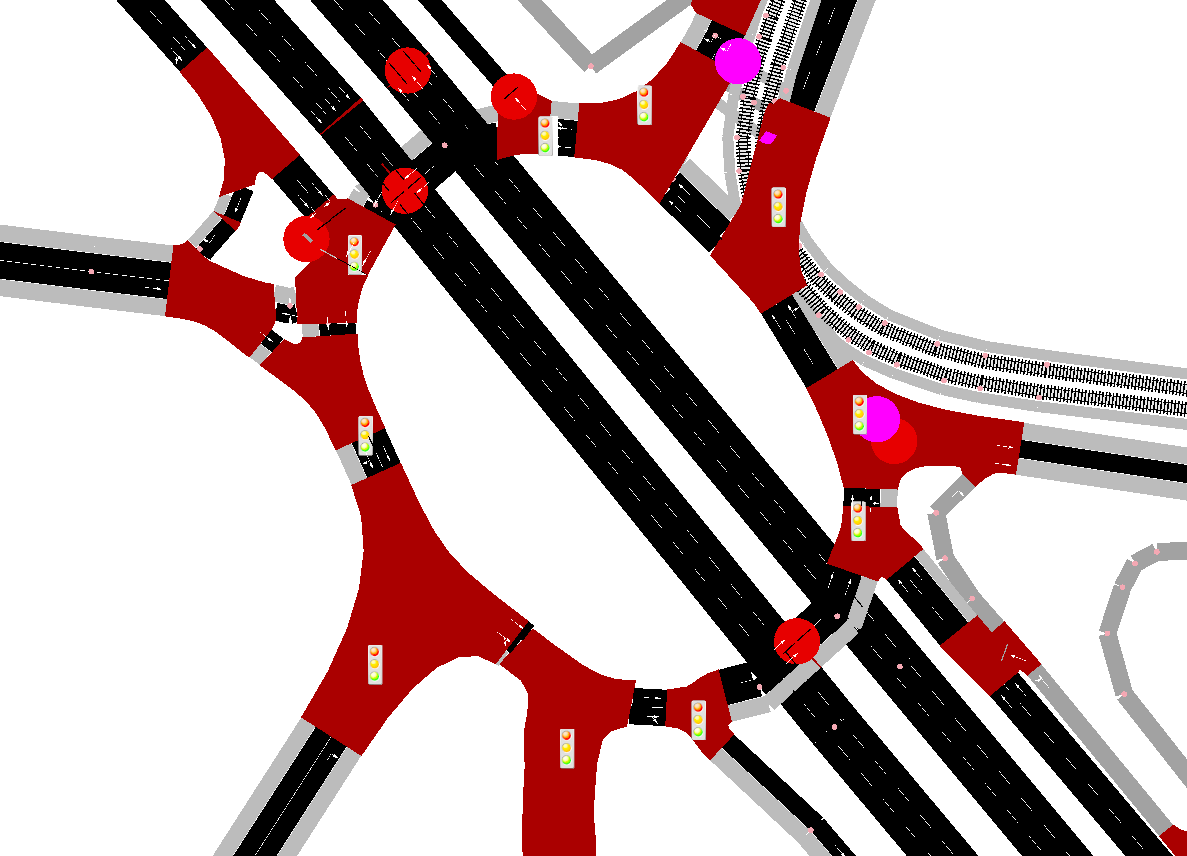
\includegraphics[width=\textwidth]{report/images/conf2.png}
        \caption{Imagen del archivo de red con los semáforos de las configuraciones 1 y 2.}
        \label{fig:conf2}
    \end{subfigure}
    \hfill
    \begin{subfigure}[t]{0.48\textwidth}
        \centering
        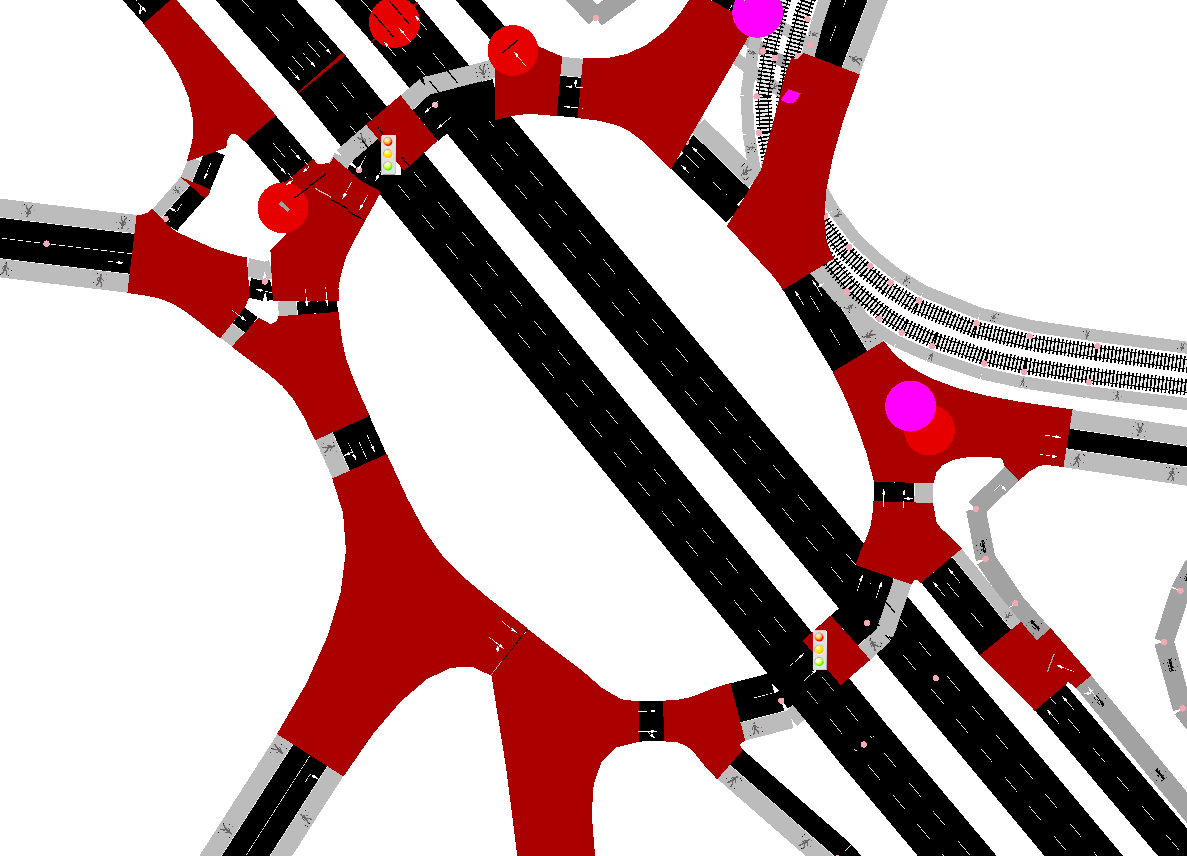
\includegraphics[width=\textwidth]{report/images/conf3.png}
        \caption{Imagen del archivo de red con los semáforos de la configuración 3.}
        \label{fig:conf3}
    \end{subfigure}
    \caption{Distintas configuraciones de los semáforos.}
    \label{fig:confs}
\end{figure}


\section{El algoritmo evolutivo}

Una vez se han definido los archivos de la simulación, corresponde evaluar la manera en que se va a implementar el algoritmo evolutivo. Para esto se ha empleado \texttt{Genetics.js}, una librería programada en TypeScript orientada a algoritmos evolutivos; en particular, algoritmos genéticos. Esta librería la programó Cristian Abrante, un antiguo alumno de la Escuela Superior de Ingeniería y Tecnología, para su TFG

\chapter{Resultados}
\label{cap:4-resultados}

Los capítulos intermedios servirán para cubrir los siguientes aspectos:
antecedentes, problemática o estado del arte, objetivos, fases y desarrollo del proyecto.




\chapter{Conclusiones y líneas futuras}
\label{cap:5-conclusiones}

Este capítulo es obligatorio.
Toda memoria de Trabajo de Fin de Grado debe incluir unas conclusiones y unas 
líneas de trabajo futuro 



\chapter{Conclusions and future work}
\label{cap:6-conclusions}

Este capítulo es obligatorio.
Toda memoria de Trabajo de Fin de Grado debe incluir unas conclusiones y unas 
líneas de trabajo futuro 



%%%%%%%%%%%%%%%%%%%%%%%%%%%%%%%%%%%%%%%%%%%%%%%%%%%%%%%%%%%%%%%%%%%%%%%%%%%%%%%
\printbibliography
% \nocite{*}

%%%%%%%%%%%%%%%%%%%%%%%%%%%%%%%%%%%%%%%%%%%%%%%%%%%%%%%%%%%%%%%%%%%%%%%%%%%%%%%
% \newpage{\pagestyle{empty}}
% \thispagestyle{empty}
% \begin{appendix}

%   \chapter{Título del Apéndice 1} 
%   \label{appendix:1}
%   \input{apendice1.tex}

%   \chapter{Título del Apéndice 2}
%   \label{appendix:2}
%   \input{apendice2.tex}

% \end{appendix}

\end{document}
